\documentclass[%
 reprint,
superscriptaddress,
%groupedaddress,
%unsortedaddress,
%runinaddress,
%frontmatterverbose, 
%preprint,
%preprintnumbers,
%nofootinbib,
%nobibnotes,
%bibnotes,
 amsmath,amssymb,
 aps,
%pra,
prb,
%rmp,
%prstab,
%prstper,
floatfix
]{revtex4-2}

\usepackage{graphicx}% Include figure files
\usepackage{dcolumn}% Align table columns on decimal point
\usepackage{bm}% bold math
%%%%%%%%%%%%%%%%%%%%%%%%%package by Zhong
\usepackage{units}
%\usepackage{lineno}
%\usepackage{float}
%\usepackage{amsmath}  % improve math presentation
%\usepackage{amsfonts}
%\usepackage{verbatim}
%%%%%%%%%%%%%%%%%%%%%%%%%%%%%%%%%%%%%%
\usepackage{hyperref}% add hypertext capabilities
\usepackage{xcolor}
\usepackage{xspace}
\usepackage{mathbbol}


\newcommand{\bjoern}[2]{{\color{blue}{{\bf #1} #2}}}
\newcommand{\ahfx}{\ensuremath{\alpha_\text{HFX}}\xspace} 


\begin{document}


\title{Uncertainty Quantification in Multiscale Models of Charge Transport in Organic Semiconductors: Influence of the Exhange-Correlation Functional}

\author{Zhongquan Chen}
\author{Pim van der Hoorn}
\author{Bj\"orn Baumeier}
\affiliation{Department of Mathematics and Computer Science \& Institute for Complex Molecular Systems, Eindhoven University of Technology}

\date{\today}

\begin{abstract}
  \bjoern{TODO}{rewrite}This work quantifies uncertainties in a multiscale model for charge dynamics in organic semiconductors (OSCs). A first-principle multiscale model integrates classical molecular dynamics (MD), density functional theory (DFT), quantum mechanical calculation and continuous-time random walk (CTRW) processes to allow the simulation of charge transport in OSCs. The model brings inherent uncertainties arising from the empirical approximations and numerical simulations. Our work particularly focusing on quantifying the uncertainty in DFT exchange-correlation functional.

  By investigating the effects of varying Hartree-Fock (HF) levels within DFT functionals, we analyze the impact on electronic structures such as reorganization energy, molecule energy distribution, and coupling elements. The primary goal is to assess the robustness of predicting the quantity of interest (QoI), that is time-of-flight and charge mobility, under these uncertainties.
  
  Monte Carlo simulations and sensitivity analysis are employed to estimate the range and confidence levels of the predicted charge mobility. As shown by Sobol indices, the QoI is most sensitive to molecule energy, then reorganization energy and least sensitive to coupling elements.  
\end{abstract}

%\keywords{Suggested keywords}

\maketitle


\section{Introduction}
Organic semiconductors (OSCs) are materials that consist of organic molecules, often in disordered structures formed during spin-coating or deposition processing. Besides their semiconducting properties, they are mechanically flexible and come with the potential to control charge transport properties~\cite{hamers_flexible_2001,liu_high_2015,chow_organic_2020}. This flexible functionality is achieved by tuning molecular properties to achieve an ideal operation at the device level~\cite{bronstein_role_2020, bredas_organic_2002}. Computational approaches that aim at predicting the charge transport properties of disordered molecular materials resolving the interplay between single-molecule properties (such as their electronic structure or response properties) and mesoscale material morphology can play an important role in supporting or even guiding experimental optimization processes~\cite{bronstein_role_2020, sokolov_computational_2011, grynova_read_2018}.\bjoern{add citations}{}

\begin{figure*}[tbp]
  \centering
  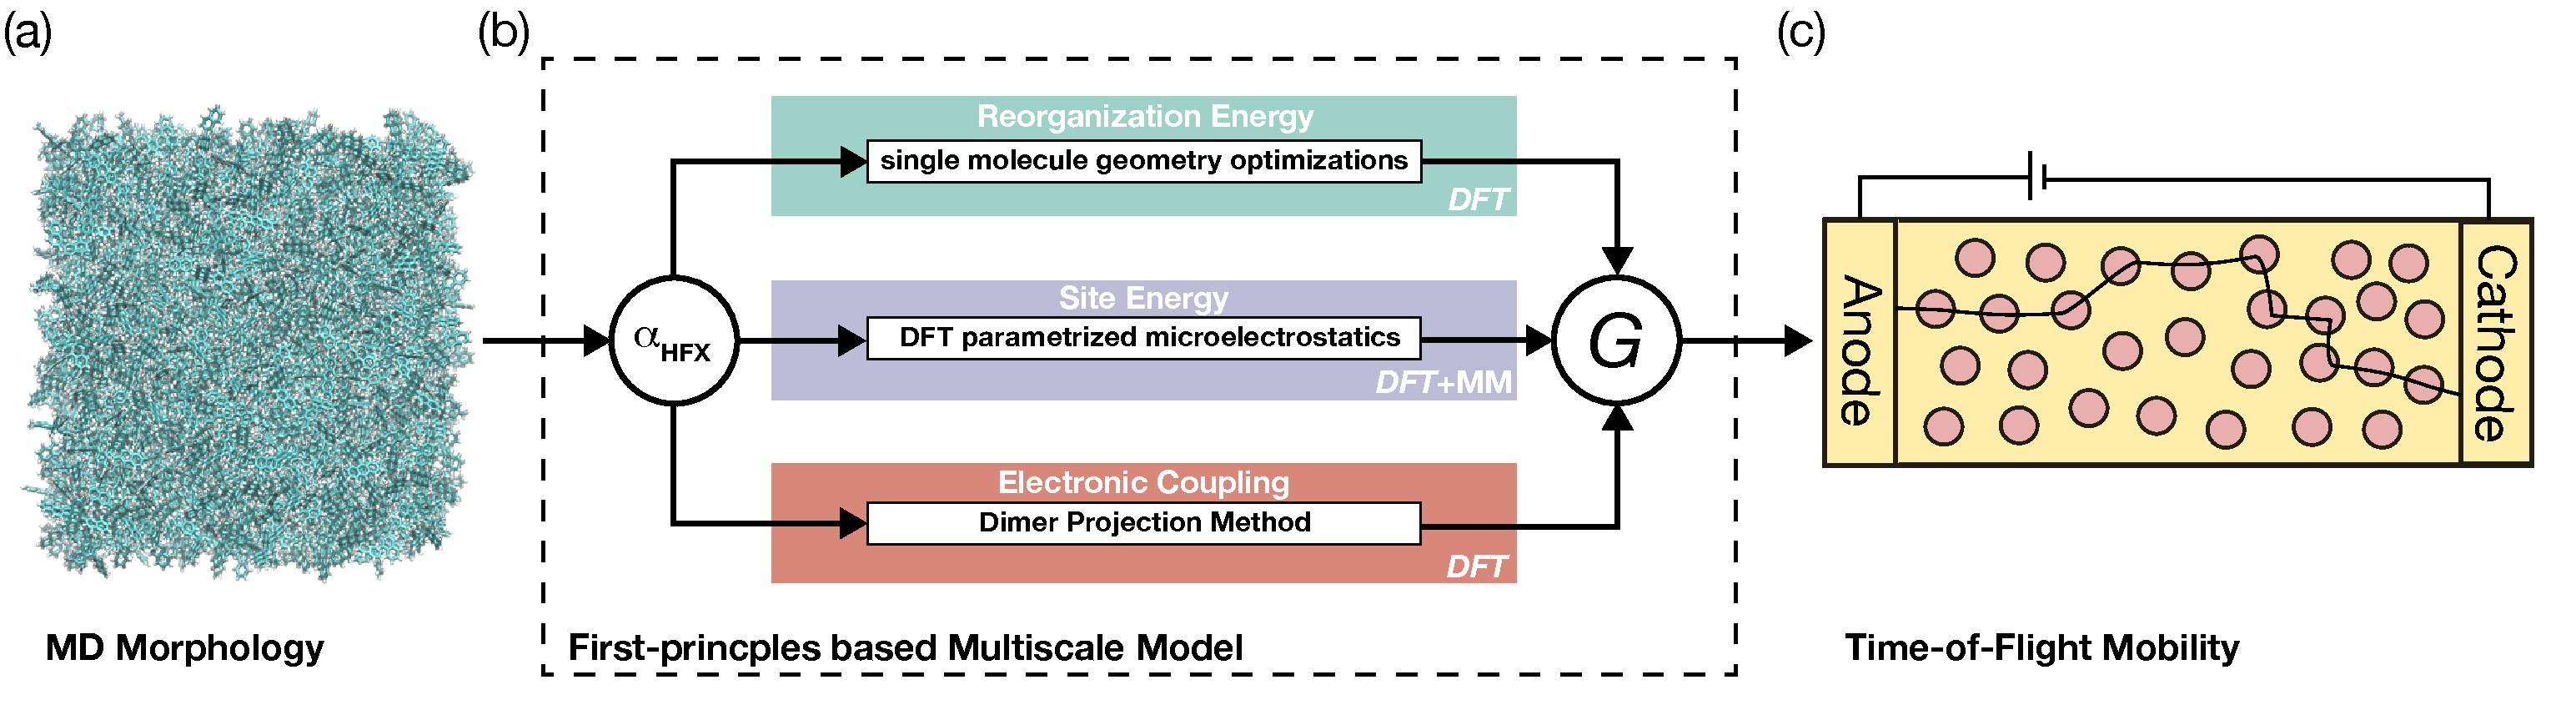
\includegraphics[width=\linewidth]{figs/MSM2.pdf}
  \caption{\bjoern{TODO Bjoern}{Rewrite caption}The multiscale model workflow for OSC. Step 1: MD simulation to generate atom coordinates. Step 2: Molecule energy $E_i$ calculation. Step 3: Calculation of Reorganization energy $\lambda_{ij}$ and coupling element $J_{ij}$ for pairs of molecule $i,j$ whose COM distance is less than $r_\text{cutoff}$. Step 4: Modelling dynamics on device level, such as ToF calculation.}
  \label{fig:MSM}
\end{figure*}

First-principles based multiscale models are such types of computational approaches. Due to the infeasibility of explicitly simulating the coupled non-adiabatic electron-nuclear dynamics for the time- and length scales of realistic materials, these models typically exploit the localization of electronic states in disordered molecular materials and consider a rate-based description of hopping-type transport. A popular choice for the electron transfer rate $\omega_{ij}$ between two localization sites $i$ and $j$ is Marcus theory~\cite{marcus_theory_1956, marcus_electron_1993}  ~\bjoern{add}{citation}, in which
%
\begin{equation}
    \omega_{ij} = \frac{2\pi}{\hbar} \frac{|J_{ij}|^2}{\sqrt{4\pi \lambda_{ij} k_\text{B}T}} \exp\left(-\frac{(\Delta E_{ij} - \lambda)^2}{4\lambda k_\text{B}T}\right) ,
    \label{equ:Marcus}
\end{equation}
%
where $\hbar$ is the reduced Planck constant,  $k_\text{B}$ the Boltzmann constant, and $T$ the temperature. As depicted in Fig.~\ref{fig:MSM}, given a larger scale morphology and with the definition of localization sites (Fig.~\ref{fig:MSM}(a)), multiscale models employ first-principles based methods (Fig.~\ref{fig:MSM}(b)) to explicitly calculate the remaining physical, material-specific (or rather transfer-pair-specific) quantities in Eq.~\ref{equ:Marcus}: the reorganization energy $\lambda$ (here a single value as we assume a single-component material), the electronic coupling $J_{ij}$, and the site energy difference $\Delta E_{ij} = E_i - E_j$. With all that information, charge transport is modeled as a continuous time random walk (CTRW) process on a graph $\mathbf{G}$, constructed from the localization sites and the calculated rates between them (Fig.~\ref{fig:MSM}(c)). Panel (b) of Fig.~\ref{fig:MSM} mentions some specific methods for the calculation of the quantities entering Eq.~\ref{equ:Marcus}, such as mixed quantum-classical methods for obtaining the site energies with the help of microelectrostatic methods~\cite{poelking_impact_2015, poelking_long-range_2016} \bjoern{add}{citations} or the dimer projection method for determining coupling elements~\cite{baumeier_density_2010}, as they are the ones adopted in this work. What is essential about these and alternative ones is that they typically rely on density-functional theory (DFT) calculations, either directly or as a mean to parametrize classical models. The dependence of DFT calculations on the choice of an exchange-correlation functional raises the question of how sensitive the simulated charge transport is to this choice and how certain predictions of material properties are. 

Uncertainty quantification (UQ) is concept from computational science which allows for an estimation of confidence intervals for a quantity of interest (QoI) and an analysis of its sensitivity in models of a physical system that contain uncertain, maybe empirical, or noisy, parameters~\cite{sarkar_uncertainty_2017,oconnor_quantifying_2024, chernatynskiy_uncertainty_2013, suleimenova_tutorial_2021,coveney_reliability_2021, coveney_when_2021}. Many common UQ studies focus on models with (partial) differential equations, e.g., drift-diffusion equations in which the diffusivity as parameter, and assume a certain distribution for the values of the parameter(s). For the multiscale model of charge transport, it is not straightforward to cast the large variety of available exchange-correlation functionals into the role of a model parameter with some distribution. To keep the problem tractable, we focus here instead specifically on the exchange part in hybrid functionals~\cite{perdew_rationale_1996,marques_densitybased_2011}, in which a DFT model for the exchange is mixed using a weighting factor $\alpha_\text{HFX}$ with a Hartree--Fock type exchange, i.e.,
%
\begin{equation}
  E_\text{x} = \alpha_\text{HFX} E_\text{x}^\text{HF} + (1-\alpha_\text{HFX})E_\text{x}^\text{DFT}.
  \label{equ:hybrid}
\end{equation}
%
More specifically, we take as the basis the PBE0 functional~\cite{adamo_toward_1999} and scrutinize (i) how the predictions of the multiscale model of charge transport are affected by variation of $\alpha_\text{HFX}$ as a proxy for uncertainties in the choice of DFT functionals, (ii) what the level of confidence is in quantitative predictions, and (iii) what are the most sensitive quantities in the model. In this sense, Eq.~\ref{equ:hybrid} is deceptively simple. For each value of $\alpha_\text{HFX}$, the graph $G$ is constructed using the respective value of the reorganization energy, the $N_\text{mol}$ site energies, and the $N_\text{pair}$ coupling elements, and the dimensionality of the problem from the perspective of UQ is $N_\text{UQ}=1+N_\text{mol}+N_\text{pair}$, which can easily be on the order of $10^{4}-10^{5}$. We consider the simulated time-of-flight (ToF) and the associated mobility the QoI in the following (see Fig.~\ref{fig:MSM}(c)) which then are subject to uncertainties in these $N_\text{UQ}$ parameters, {\em stemming} from the variation in $\alpha_\text{HFX}$. As a prototypical system, we will study hole transport in an amorphous morphology of 2-methyl-9, 10-bis(naphthalen-2-yl)anthracene (MADN), a wide-gap semiconductor that is used extensively as an ambipolar host material in organic light-emitting diodes~\cite{ko_accurate_2019, chang_great_2017} ~\bjoern{add}{citation}. 

This paper is organized as follows. Section~\ref{sec:model} outlines the theoretical and computational details of the multiscale model, including the morphology simulation with classical molecular dynamics, the determination of all quantities in the transition rates, and the calculation of the charge transport properties from the constructed graph model. In Section~\ref{sec:MSMresults}, we discuss the explicit results from the model using different values of $\alpha_\text{HFX}$, before we show the results of uncertainty quantification and sensitivity analysis via Monte Carlo sampling. A brief summary concludes the paper. 

\section{Multiscale Model}
\label{sec:model}
The multiscale model maps a large scale molecular morphology with atomistic detail into a graph $\mathbf{G}(\mathbf{V}, \mathbf{W})$, where the set of nodes $\mathbf{V}$ is determined from the center-of-masses of the individual molecules and $\mathbf{W}$ is the adjacency matrix formed by the Marcus rates $\omega_{ij}$. Two nodes $i,j$ are connected if the corresponding molecules have their closest-contact distance smaller than $r_\text{cutoff}=\unit[0.5]{nm}$. 

\subsection{Molecular Dynamics}
Classical molecular dynamics (MD) is used to create an amorphous morphology of MADN. An empirical force-field for these simulations has been obtained via the Automated Topology Builder~\cite{stroet_automated_2018}, and an initial structure containing 1000 molecules in a cubic cell is created. Periodic boundary conditions are applied throughout in all three spatial directions. 
After energy minimization, the system is simulated for \unit[1]{ns} in the $NpT$ ensemble, keeping a constant temperature of \unit[300]{K} and constant pressure of \unit[1]{bar} using the velocity-rescale thermostat~\cite{bussi_canonical_2007} with the coupling time constant \unit[0.1]{ps} and the Parrinello-Rahman barostat~\cite{parrinello_polymorphic_1981} with a time constant for pressure coupling \unit[2]{ps}. The equation of motion for updating the atomic coordinates is implemented by leap-frog algorithm~\cite{van_gunsteren_leap} with a time step of \unit[1]{fs}. Following this, the temperature is increased to \unit[800]{K}, well above the glass transition temperature, during a period of \unit[0.5]{ns}. This temperature is maintained for \unit[1]{ns} before cooling back down to \unit[300]{K} during a period of \unit[0.5]{ns}. Such a heating-cooling cycle is repeated three times. After this simulated annealing, a production run is conducted for \unit[2]{ns} using the $NpT$ ensemble. The final configuration of MADN is chosen for the further steps in the multiscale model, whose configuration is a cubic box with a length of \unit[9.0]{nm} and a density of $\unit[1.08]{g/cm^3}$. All calculations have been performed with the GROMACS software package~\cite{berendsen_gromacs_1995}.

\subsection{Electronic Structure Calculations} 
\label{sec:es}
Molecular orbitals $\phi_l (\mathbf{r})$ with energies $\epsilon_l$ of the individual molecules in the morphology are obtained within DFT as the solutions to the  Kohn--Sham equations~\cite{kohn_self_1965}
%
\begin{eqnarray}
    && \left(-\frac{1}{2}\nabla^2_{\mathbf{r}} + v_\text{ext}(\mathbf{r}) + v_\text{H}[\rho](\mathbf{r}) + v_\text{XC}[\rho](\mathbf{r})\right) \phi_l(\mathbf{r}) \nonumber \\
    && = H^\text{KS} \phi_l(\mathbf{r}) = \epsilon_l \phi_l (\mathbf{r}) ,
    \label{eq:KS2}
\end{eqnarray}
%
where $v_\text{ext}$ in an external potential (typically from the nuclei), $v_\text{H}[\rho]$ the electrostatic Hartree potential of a classical charge density $\rho(\mathbf{r})$, and $v_\text{XC}[\rho]$ the exchange-correlation potential containing explicit quantum-mechanical electron-electron interactions. The charge density is determined from the single-particle wave functions as $\rho(\mathbf{r})=\sum\limits_{l=1}^{N_\text{el}} \left\vert\phi_l(\mathbf{r})\right\vert^2$. As the Hartree and exchange-correlation potential depend on this density, solutions to Eq.~\ref{eq:KS2} have to be found self-consistently. This corresponds to finding the ground-state density $\rho_0$ that minimizes the total energy of the system expressed as
%
\begin{equation}
    U=U[\rho] = T_s[\rho] + \int v_\text{ext}(\mathbf{r}) \rho(\mathbf{r}) d \vec{r} + E_\text{H}[\rho] + E_\text{XC}[\rho]
    \label{eq:KS_model}
\end{equation}
%
where $T_s[\rho]$ is the kinetic energy, $E_\text{H}[\rho]$ and $E_\text{XC}[\rho]$ the Hartree and exchange-correlation energies, respectively. 

The practical calculations in this work have been performed with the ORCA software~\cite{Neese2012a} using the def2-tzvp~\cite{weigend_accurate_2006} basis set to represent the Kohn--Sham wave functions. As mentioned in the Introduction, the correlation part of the exchange-correlation functional is taken from the PBE0 functional, while the weighting factor of the Hartree--Fock type exchange in the exchange part is varied. In common practice, $\alpha$ is small and below 0.25. For our uncertain quantification study, $\alpha=0,0.05,0.10,0.15,0.20,0.25$ are chosen for the multiscale model.

\subsection{Reorganiztion Energy}
 The reorganization energy $\lambda$ accounts for the energy change caused by the geometry variation during the charge transport, and is linked to four points on the potential energy surfaces of neutral (n) and charged (c) molecules at neutral (N) or charged (C) equilibrium geometries via:
%
\begin{equation}
    \lambda_{ij} = U_i^\text{nC} - U_i^\text{nN} + U_j^\text{cN} - U_j^\text{cC},
    \label{eq:lambda}
\end{equation}
%
where $U^\text{xX}$ is the total DFT energy of $\text{x}=\text{n},\text{c}$ state in the $\text{X}=\text{N},\text{C}$ geometry. While in principle transfer pair specific, we use a single value of all molecular pairs.

\subsection{Site Energy}
The site energy $E_i = E_i^\text{c} - E_i^\text{n}$ is the difference between the total energies of the system in which molecule $i$ is carrying a charge or not, corresponding to the ionization potential in case of hole transport and the negative of the electron affinity in case of electron transport. The individual total energies in turn consist of different contributions associated with different physical mechanism, i.e.,
%
\begin{equation}
E_i^x = U_i^\text{xX} + E_i^{\text{x},\text{el}} + E_i^{\text{x},\text{polar}},
\label{eq:Es}
\end{equation}
%
where $U_i^\text{xX}$ is the internal energy contributions and both $E_i^{\text{x},\text{el}}$ and $E_i^{\text{x},\text{polar}}$ are contributions arising from purely static and polarizable intermolecular interactions, respectively. As those interactions are typically long-ranged, the intermolecular contributions to the site energy can typically not be calculated with a fully quantum-mechanical method and classical models are adopted, instead, which we refer to as a microelectrostatic model using moment representations parametrized based on single molecule DFT reference data. Specifically, in the multiscale model here, we employ a point charge respresentation~\cite{jcc540110311} for the electrostatic potential of charged and neutral molecules, so that the electrostatic energy contribution is
%
\begin{equation}
    E_i^{\text{x},\text{el}} = \frac{1}{4 \pi \epsilon_0} \sum\limits_{a_i} \sum\limits_{b_k,k \neq i} \frac{q^\text{x}_{a_i}q^n_{b_k}}{ |\mathbf{R}_{a_i} - \mathbf{R}_{b_k}|} 
\end{equation}
%
where $\epsilon_0$ is the vacuum permittivity, $a_i, b_k$ denotes the atoms in molecule $i,k$, $q^{\text{x}}_{a_i}$ are the partial charge of atom $a$ when molecule $i$ is in state $\text{x}$. To account for effects of polarization, and to evaluate $ E_i^{\text{x},\text{polar}}$, we use the model of distributed atomic dipole polarizabilities (Thole model)~\cite{thole_molecular_1981}, in which the parameters are also determined such that the classical volume of the molecular polarizability tensor matches the DFT reference.
Intermoelcular effects are considered in a region of \unit[4.0]{nm} around each individual molecule. Practical calculations of the site energies are performed using the VOTCA software~\cite{Baumeier2011,doi:10.1021/acs.jctc.8b00617,10.1063/1.5144277,Baumeier2024}.

\subsection{Electronic Coupling Elements}
The coupling element $J_{ij}$ between molecule $i$ and $j$ describe the coupling strength between two localized states, here approximated by monomer single-particle wavefunctions $\vert \phi_i\rangle$ and $\vert\phi_j\rangle$, respectively. For hole transport, the relevant orbitals are highest-occupied molecular orbital (HOMO). Using the Dimer-Projection Method~\cite{baumeier_density_2010} the coupling element is determined as:
%
\begin{equation}
    J_{ij} = \frac{ J^0_{ij}- \frac{1}{2}(e_i+e_j) S_{ij} }{ 1- S_{ij}^2 }
    \label{equ:JAB}
\end{equation}
%
where $J^0_{ij} = \langle \phi_i | \hat{H}^\text{KS}_\text{D} | \phi_j \rangle $, $e_i = \langle \phi_i | \hat{H}^\text{KS}_\text{D} | \phi_i \rangle $, $e_j = \langle \phi_j | \hat{H}^\text{KS}_\text{D} | \phi_j \rangle $, and $S_{ij}=\langle \phi_i | \phi_j \rangle $ with bra-ket notation. The Hamiltonian of the dimer,  $H^\text{KS}_\text{D}$ (see Eq.~\ref{eq:KS2}), is diagonal in its eigenbasis $\left\{\vert \phi^\text{D}_k\rangle\right\}$ with eigenvalues $\left\{ \epsilon^\text{D}_k\right\}$, so $H^\text{KS}_\text{D} = \text{diag}(\epsilon^\text{D})$. With the projections of the monomer functions on the dimer eigenbasis, i.e., $p_{ik} = \langle \phi_i | \phi^\text{D}_k \rangle$ and  $p_{jk} = \langle \phi_j | \phi^\text{D}_k \rangle$, $J^0_{ij}$ can be calculated as $J^0_{ij} = \mathbf{p}_i^\text{T} \text{diag}(\epsilon^\text{D}) \mathbf{p}_j$. Similarly, $e_{i(j)} = \mathbf{p}_{i(j)}^\text{T} \mathbf{p}_{i(j)}$ and $S_{ij} =  \mathbf{p}_i^\text{T} \mathbf{p}_j$. All  of these operations are performed in the basis set representation of the Kohn--Sham wave functions (see Sec.~\ref{sec:es}) as implemented in VOTCA.

\subsection{Time-of-flight Calculation}
After constructing the  graph $\mathbf{G}$ from the multiscale model, charge dynamics are modeled as a continuous-time random walk on this graph. In the time-of-flight (ToF) model, some vertices serve as source nodes, representing the electrode where charge carriers are injected, and some as sink nodes, where charge carriers are detected and the ToF is recorded. In CTRW the ToF is calculated as the expected hitting time of a continuous time Markov chain. For a system with $N$ molecules and one charge carrier, the transition rates between the molecules define the adjacency matrix $\mathbf{W}$:
%
\begin{equation}
  \label{eq:transition_rates}
	\mathbf{W}_{ij} =
	\begin{cases}
	     0			&  i \text{ is not connected to } j,\\
         \omega_{ij}   &  i \text{ is connected to } j,
	\end{cases}
\end{equation}

Then the transition probability from state $i$ to $j$ is $p_{ij} = \mathbf{W}_{ij}/D_i$ where $D_i := \sum_{j} \mathbf{W}_{ij}$.
And the expected time from node $i$ to reach the sink $\tau_i$ is calculated via: 
%
\begin{equation}
  \label{eq:hitting_time}
	\tau_i = \begin{cases}
		\frac{1}{D_i} + \sum_{j \ne i} p_{ij} \tau_{j} &\text{if $i$ is not a sink node},\\
		0 &\text{else.} 
	\end{cases}
\end{equation} 

To account for all possible starting nodes of the carrier, all source nodes must be considered. The random walk process can be modeled as a parallel electric network of capacitors~\cite{doyle_random_1984}. Accordingly, the ToF is evaluated using the harmonic mean:
%
\begin{equation} 
  \tau = N_\text{source} \left[\sum_{i \in \text{Source}} (\tau_i)^{-1}\right]^{-1},
  \label{eq:ToF}
\end{equation}
%
where $N_\text{source}$ is the number of source nodes.

To determine the ToF in the simulated MADN system along the positive $x$-direction, we remove the PBC in this direction and define the nodes with coordinates $\unit[0]{nm} < x < \unit[0.5]{nm}$ as source nodes, and those with coordinates $\unit[8.5]{nm} < x < \unit[9]{nm}$ as sink nodes. These definitions are changed accordingly for simulating transport in negative $x$-direction, and $y$- or $z$-directions.

\section{Explicit Results from the Multiscale Model}
\label{sec:MSMresults}
In this section, we present and analyze the explicit results of the multiscale model of charge transport in amorphous MADN as obtained for different values of $\alpha_\text{HFX}$.



\subsection{Molecular Parameters}

\begin{figure}[tbp]
    \centering
    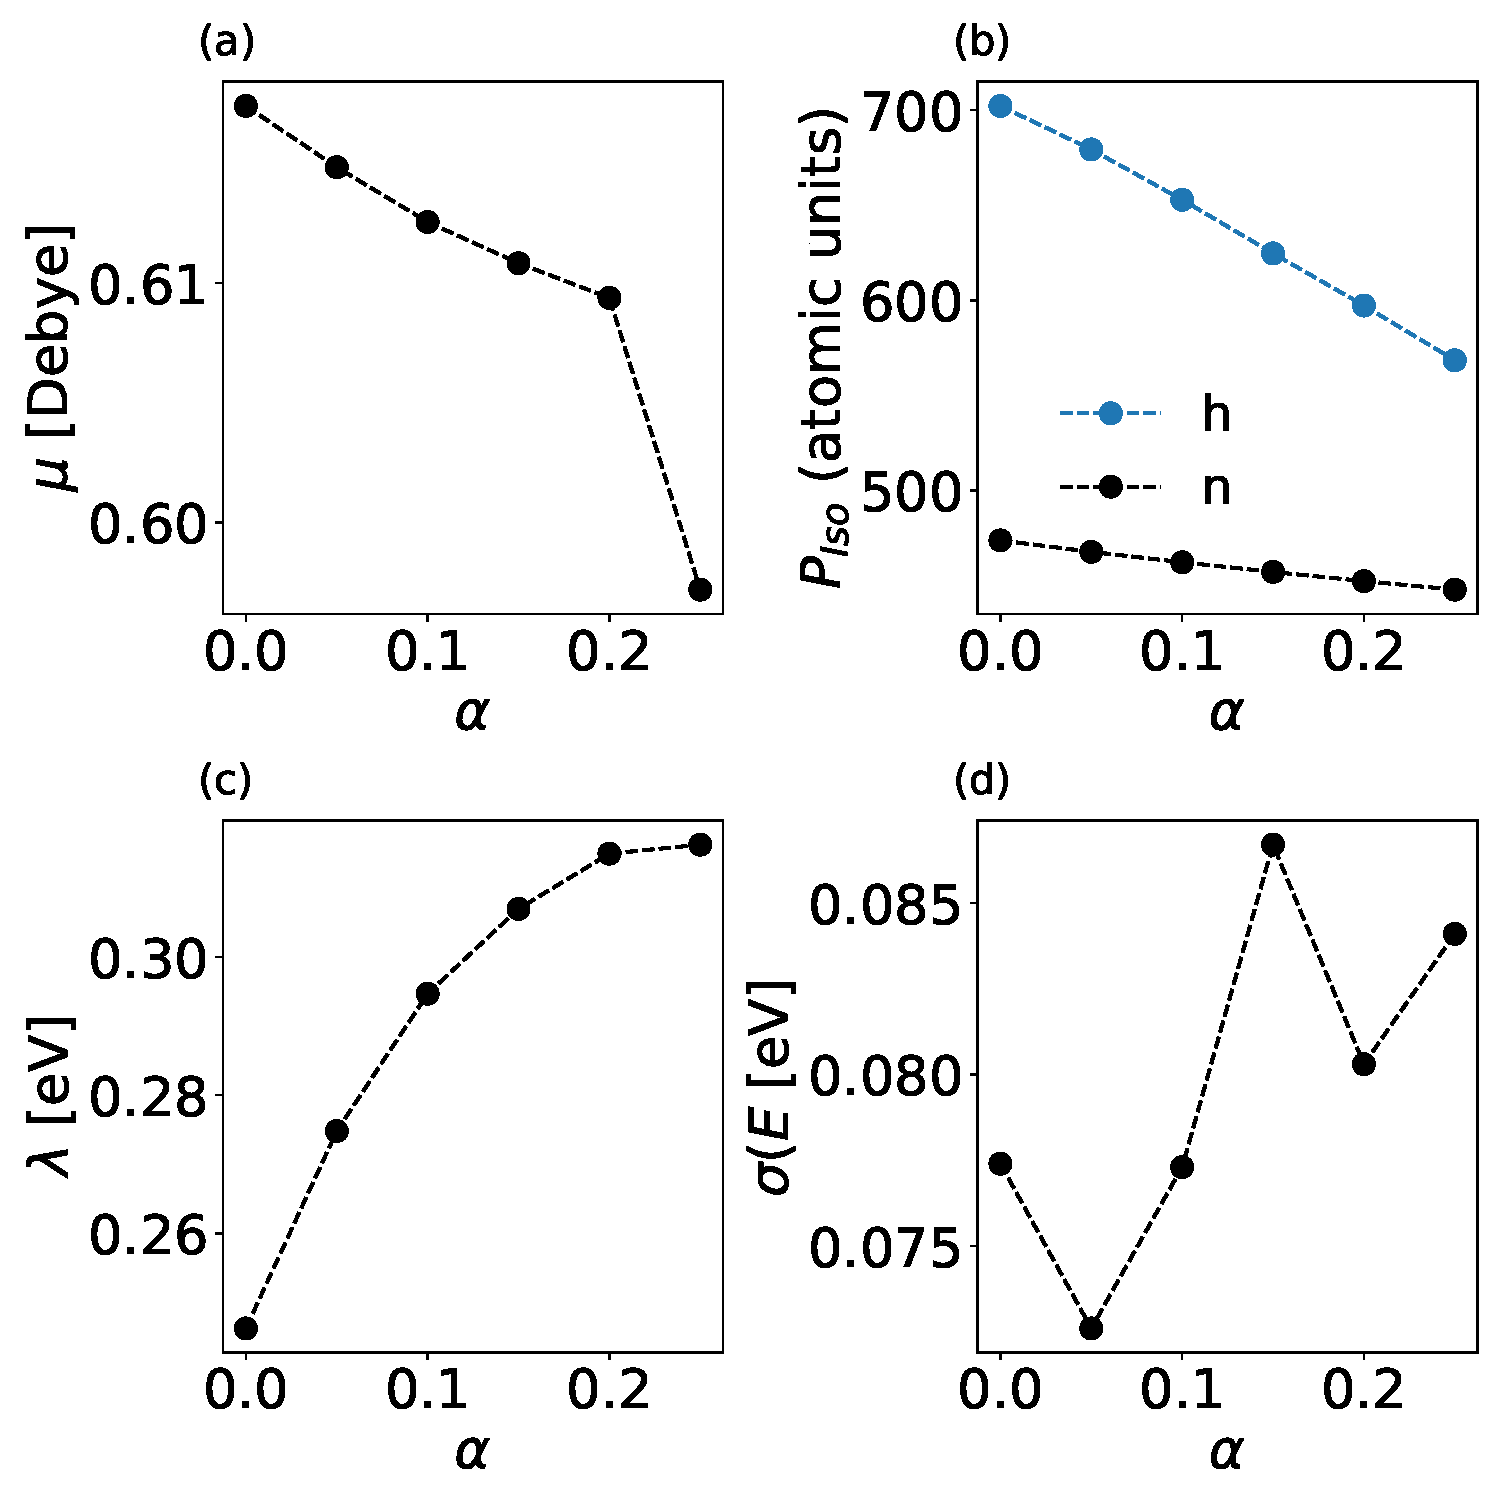
\includegraphics[width=\linewidth]{figs/fig_autogen.pdf}
    \caption{Dependence of molecular parameters as used directly in the multiscale model or in its paramaterization phase on the amount of Hartree--Fock type exchange in the PBE0-based hybrid functional $\alpha_\text{HFX}$. (a) The adiabatic ionization potential, (b) reorganization energy, (c) dipole moment of the neutral molecule, and (d) isotropic molecular polarizability in neutral and charged states, respectively.}
    \label{fig:autogen_MADN}
\end{figure}

We begin with a brief discussion of the molecular parameters as they are used in different ways in the multiscale model. Figure~\ref{fig:autogen_MADN} shows the adiabatic ionization potential, reorganization energy, neutral state dipole moment, and isotropic polarizability in neutral and cationic (hole) states, respectively. The adiabatic ionization potential in Fig.~\ref{fig:autogen_MADN}(a) in principle contributes to the site energy but as it is determined per molecule-type in the system, it has no effect on the site-energy difference $\Delta E_{ij}$ in Eq.~\ref{equ:Marcus}. It is nevertheless interesting to see that it increases almost linearly over the shown range of \ahfx. In contrast, the reorganization energy as shown in Fig.~\ref{fig:autogen_MADN}(b) appears to saturate for \ahfx after an initially close to linear increase. In total, $\lambda$ is found to be in an interval between \unit[0.246]{eV} and \unit[0.316]{eV} \bjoern{need}{correct numbers here}. Panels (c) and (d) of Fig.~\ref{fig:autogen_MADN} show the dipole moment of the neutral MADN molecule and the isotropic polarizability of the neutral and cationic (hole) states, respectively, both as electrostatic properties that enter indirectly the parameterization of the microelectrostatic model. As is visible, the dipole moment is rather independent on \ahfx (note that the jump of the last shown data point appears more pronounced because of the vert small scale on the $y$-axis). The isotropic polarizabilities in panel (d) exhibit a linear decrease with increasing value of \ahfx which can be attributed to an increasingly attractive effective potential from stronger the Hartree--Fock-like exchange term and consequently more strongly bound electrons as one can also see from the increaseing ionization potential in panel (a).  

\subsection{Site energies}

\begin{figure*}[tbp]
  \centering
  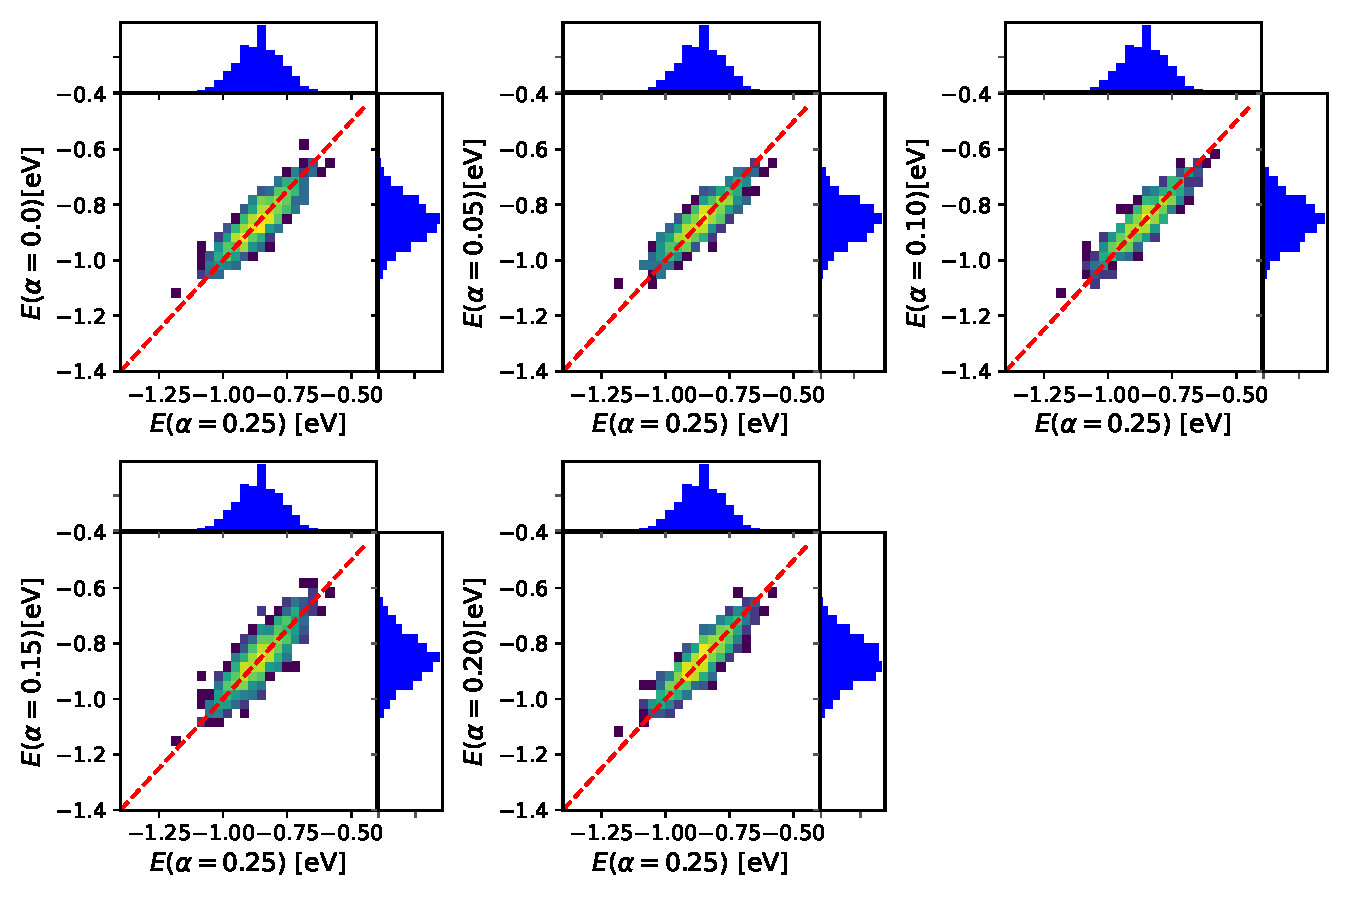
\includegraphics[width=\linewidth]{figs/scatterE_qmmm.pdf}
  \caption{\bjoern{TODO: }{rewrite caption}Scatter plot of site energy of MADN molecules calculated from different HFX, compared to the site energy calculated from HFX=0.25 (The PBE0 functional). The brighter color near the diagonal lines indicates denser population of the molecules.  The top and right histogram show the energy distributions.}
  \label{fig:E_qmmm_MADN}
\end{figure*}

\begin{table}[tbp]
  \caption{\bjoern{TODO: }{rewrite caption}In the tested $\alpha'$ values, the second column shows the maximum of $E_i(\alpha=0.25) - E_i(\alpha')$ for all molecules. Denoting $i'$ as the index of the molecule which has maximum $E_i(\alpha=0.25) - E_i(\alpha')$ for the chosen $\alpha'$, the third column shows the energy of molecule $i'$ calculated by $\alpha=0.25$. The fourth column shows the molecule energy $E_{i'}(\alpha')$ calculated by $\alpha'$. All the energies are in unit $\unit[]{eV}$.}
  \begin{ruledtabular}
    \begin{tabular}{c c c c c c c}
    $\ahfx$ & $E_\text{min}$ & $E_\text{max}$ & $\sigma$ & $\sigma_\text{el}$ & $\sigma_\text{polar}$ &  $D_{\ahfx}$ \\%  & $E_{i_\text{max}}$ \\
    \hline
    0    & -1.11 & -0.59 & 0.08 & 0.10 & 0.04 & 0.13 \\ %&  -0.94 \\
    0.05 & -1.07 & -0.63 & 0.07 & 0.09 & 0.04 & 0.12 \\ %&  -0.94 \\
    0.10 & -1.13 & -0.61 & 0.08 & 0.10 & 0.04 & 0.13 \\ %&  -0.94 \\
    0.15 & -1.16 & -0.59 & 0.09 & 0.11 & 0.05 & 0.15 \\ %&  -0.69 \\
    0.20 & -1.12 & -0.63 & 0.08 & 0.10 & 0.05 & 0.12 \\ %&  -0.82 \\
    0.25 & -1.17 & -0.60 & 0.08 & 0.11 & 0.04 & ---  \\ %&   ---\\
    \end{tabular}
  \end{ruledtabular}
  \label{tab:maxEi}
\end{table}

Figure~\ref{fig:E_qmmm_MADN}(a)-(e) presents scatter plots comparing the distributions of the calculated site energies of MADN molecules for different \ahfx values, using $\ahfx = \unit[0.25]{}$ (PBE0 functional) as a reference in all cases. Visually, the distributions look very similar as most data points cluster near the diagonal line. In Table~\ref{tab:maxEi}, we report the minimum ($E_\text{min}$) and maximum ($E_\text{max}$) values of the energies and the standard deviation $\sigma$ of the individual distributions, which are also shown in Fig.~\ref{fig:E_qmmm_MADN}(f). All noted variations in these quantities appear small. The data in Figures~\ref{fig:Estat_qmmm_MADN} and \ref{fig:Edip_qmmm_MADN} in the Appendix show that the observations on the total site energies also hold for the individual contributions of electrostatic and polarization energies. This is also reflected by the small variations in the respective standard deviations $\sigma_\text{el}$ and $\sigma_\text{polar}$ listed in Tab.~\ref{tab:maxEi}.

Interestingly, we find the biggest variation of \unit[0.1]{eV} in the values for $E_\text{min}$. This minimal energy (or rather all the energies in the low-energy region of the distributions) can have a very significant influence on the charge transport properties, depending on how much the site energy differences are influenced in the charge transport network. To further characterize the effect of different \ahfx values, we consider the largest absolute variation in the site energies depending on \ahfx by calculating the Chebyshev distance $D_{\ahfx} = \max\limits_{i}(|E_i(\ahfx=0.25) - E_i(\ahfx)|)$. From the results listed in Tab.~\ref{tab:maxEi}, one can see that on individual level the site energies can vary substantially, with more than \unit[0.1]{eV}. This variation is larger than the recorded values of $\sigma$ and with all \ahfx yielding the same mean site energy of \unit[-0.86]{eV} this could indicate non-neglibible effects on charge transport. 

\subsection{Electronic couplings}

\begin{figure*}[tbp]
  \centering
  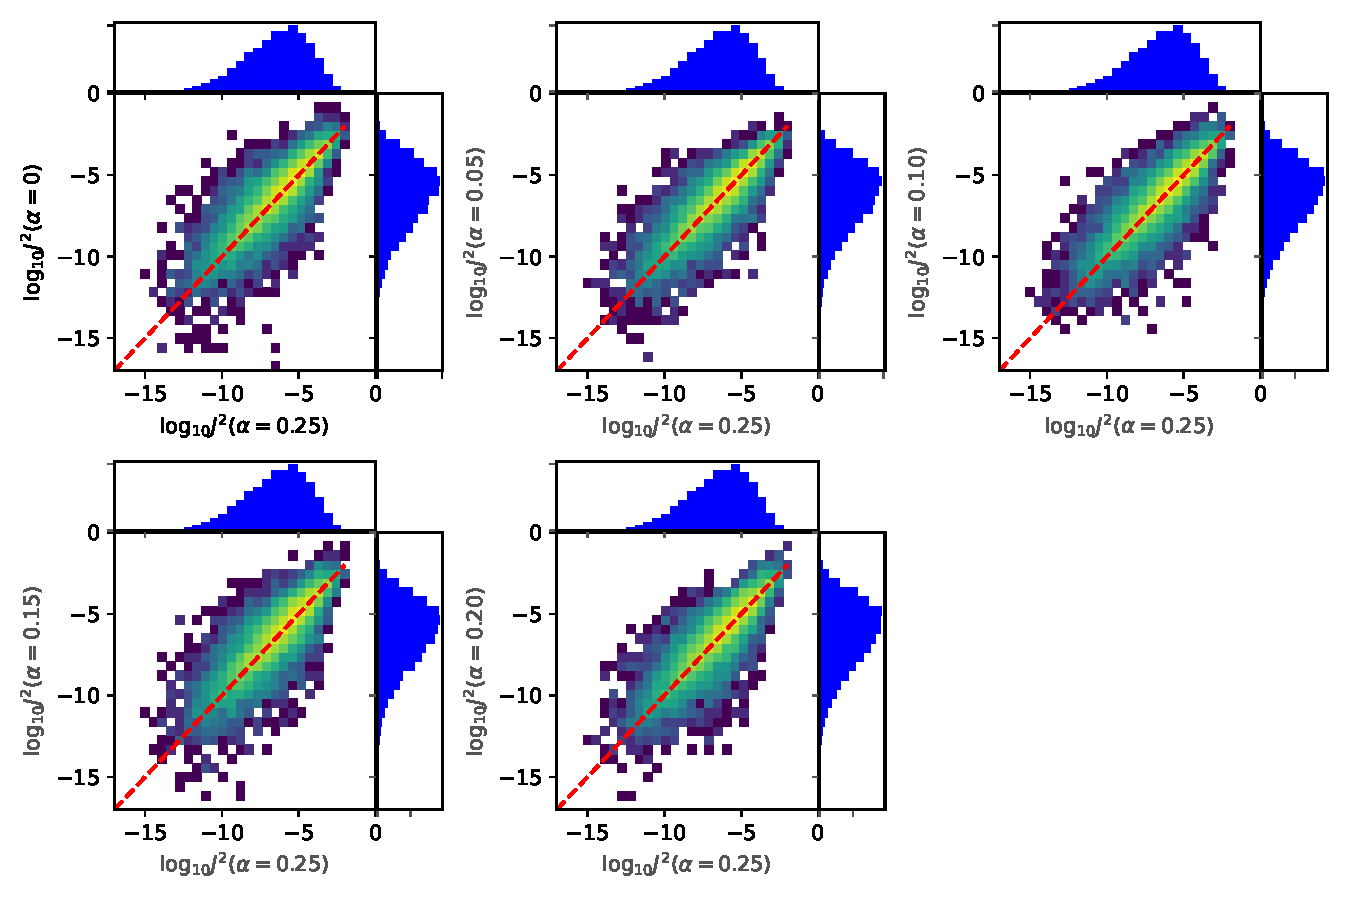
\includegraphics[width=\linewidth]{figs/scatterJ_all.pdf}
  \caption{\bjoern{TODO:}{rewrite caption} Scatter plot of MADN coupling element $\log_{10} J^2$ calculated from different HFX, compared to the polarization energy calculated from HFX=0.25 (The PBE0 functional). The brighter color near the diagonal lines indicates denser population of the molecules.  The top and right histogram show the energy distributions.}
  \label{fig:J_MADN}
\end{figure*}

Distributions and correlations compared with the PBE0 reference for the electronic coupling elements calculated with different values for \ahfx are shown in Figure~\ref{fig:J_MADN}. The individual distributions appear very similar, with a peak of $\log_{10}[(J_{ij}/\unit[]{eV})^2]$ between \unit[-5]{} to \unit[-6]{}, and a long tail of the distribution towards more negative values. The comparison with the PBE0 reference shows that while there is a clear correlation between the results for different values of \ahfx, the spread in the order of magntitudes of $J_{ij}^2$ can be very large especially for the lower coupling regions. Overall, the squared electronic coupling elements are found in a very wide range from $\unit[10^{-2}]{}$ to $\unit[10^{-15}]{(eV)^2}$ due to its exponential distance dependence and sensitivity to mutual orientation of the two involved molecules. Whereas the site energy distributions discussed in the preceding section are well-defined in the sense that each energy is unambiguously associated to a physical entity -- a molecule in the morphology --, the coupling elements are evaluated for a neighborlist based on a chosen cutoff as explained in Section~\ref{sec:model}.\bjoern{TODO:}{add!} Clearly, if this cutoff is chosen to be large, a lot of hopping pairs with very small coupling elements will be considered that may not be relevant at all (or even unphysical) for charge transport. Therefore, the increasing deviations for the most negative values in Figure~\ref{fig:J_MADN} may not be relavent either. 

\begin{figure}[tbp]
  \centering
  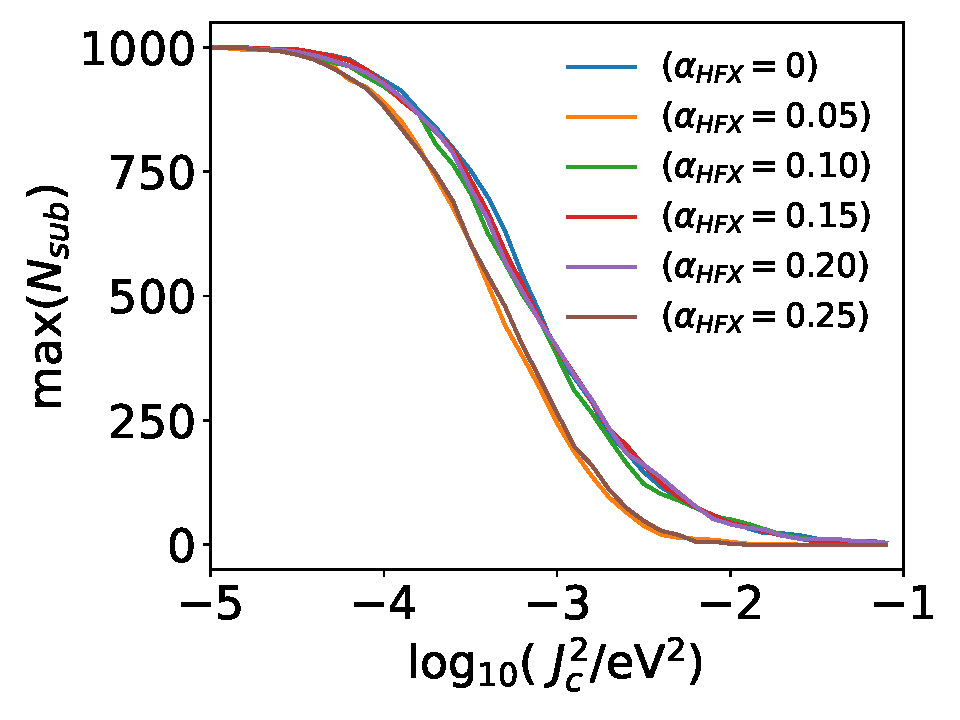
\includegraphics[width=\linewidth]{figs/fig_network_all.pdf}
  \caption{\bjoern{TODO Zhong:}{same comments regarding the $\log_{10}$ as above; replace $\alpha$ with $\alpha_\text{HF}$.}The maximum size of the subgraphs obtained in the percolation algorithm as a function of critical value $J_c$. The molecular systems obtained by different HFX are colored according to the legend.}
  \label{fig:J_percolate}
\end{figure}

To determine the range of $\log_{10}[(J_{ij}/\unit[]{eV})^2]$ that are significant for the charge dynamics, a percolation analysis is performed to find a critical threshold value for the squared electronic coupling below which the largest connected subgraph is identical to the full graph. This is achieved by removing for a given value for $J_\text{c}$ from the full graph the edges with $J_{ij}^2 < J^2_\text{c}$ followed by the determination of the number of vertices in the larges connected subgraph $\max(N_\text{sub})$. Figure~\ref{fig:J_percolate} shows the resulting dependence of $\max({N_\text{sub}})$ on the critical value $J_c$. It is apparent that for $\log_{10} J_c^2 = -5$, all vertices are in the largest connected subgraph. The overall connectivity of the charge transport network is therefore mostly affected by the coupling elements larger than this threshold, and the charge transport properties are expected to be more sensitive to deviations for the associated edges. We also note that overall, the results in Fig.~\ref{fig:J_percolate} again seem to be very similar for all \ahfx studied in the work. 


\subsection{Time-of-flight calculations}


\begin{table}[tbp]
\caption{\bjoern{TODO:}{rewrite}The ToF and diffusive velocity calculated by ToF along a distance $L_x = \unit[9.0]{nm}$ with and without energy disorder of the MADN system as a function of the HFX. The ToF is in unit $\unit[]{s}$ and $v_\text{ToF}$ in unit $\unit[]{m/s}$.}
\begin{ruledtabular}
  \begin{tabular}{c c c c }
        \ahfx & full & $J_{ij} \mathbb{1}(\log_{10} J^2_{ij} > -5)$ & $\Delta E_{ij} =0$ \\% & $v_\text{ToF}$(no $E$) \\
    \hline
        0.00 &  $6.4 \cdot 10^{-9}$ & $7.5 \cdot 10^{-9}$ & $1.9 \cdot 10^{-10}$ \\%& 42 \\
        0.05 & $ 7.9 \cdot 10^{-9}$ & $8.1 \cdot 10^{-9}$ & $4.1 \cdot 10^{-10}$ \\%& 20 \\
        0.10 & $ 1.6 \cdot 10^{-8}$ & $1.6 \cdot 10^{-8}$ & $4.0 \cdot 10^{-10} $ \\%& 20 \\
        0.15 & $ 3.0 \cdot 10^{-8}$ & $3.1 \cdot 10^{-8}$ & $4.0 \cdot 10^{-10} $ \\%& 25 \\
        0.20 & $ 2.1 \cdot 10^{-8}$ & $2.5 \cdot 10^{-8}$ & $4.5 \cdot 10^{-10}$ \\%& 18 \\
        0.25 & $ 9.5 \cdot 10^{-8}$ & $9.7 \cdot 10^{-8}$ & $7.2 \cdot 10^{-10}$ \\%& 11 \\
    \end{tabular}
\end{ruledtabular}
\label{tab:ToF_MADN_HFX}
\end{table}

From the analysis of reorganization energies, site energies, and electronic coupling elements for different values of \ahfx, it is not clear how the mostly on distribution-level observed variations impact the overall charge transport properties. To scrutinize the dependence of such a material property, we now calculate the time-of-flight $\tau$ and report the respective values in Table~\ref{tab:ToF_MADN_HFX}. Here, we refer with ''full'' to time-of-flight obtained for the the as-calculated charge transport network. One can see that $\tau$ varies by roughly one order of magnitude between $\ahfx=0$ ($\unit[6.3\cdot 10^{-9}]{s}$) and $\ahfx=0.25$ ($\unit[9.5\cdot 10^{-8}]{s}$), with an almost monotonous increase. When the squared coupling elements with values below $\unit[10^{-5}]{(eV)^2}$ are set to zero ($J_{ij} \mathbb{1}(\log_{10} J^2_{ij} > -5)$), one obtains only minimally, but consistently, larger $\tau$, corroborating the notion that the very small coupling elements are of little relevance for charge transport. Finally, we also consider the case in which the energetic disorder is ignored ($\Delta E_{ij}=0$). Here, one also can see (next to the generally shorter time-of-flight) a consistent increase in $\tau$, however only by a factor of about \unit[3.8]{}, a combined effect of the increased reorganization energy and variations in coupling elements.



%%%%%%%%%%%%%%%%%%%%%%%%%%%%%%%%%%%%%%%%%%%%%%%%%%%%%%%%%

\section{Uncertainty Quantification and Sensitivity Analysis}
\label{sec:UQ}
The previous section shows that different HFX affect the calculated ToF. In this section, we use the Monte Carlo method to estimate the range of the ToF given a confidence level, followed by a sensitivity analysis to determine which parameter contributes more to the variance of ToF. 

\subsection{Monte-Carlo Sampling of ToF}
As discussed the ToF is calculated from the graph with weighted edges defined by the electronic structure data $(\lambda, E_1,\ldots,E_N, J_1^2,\ldots,J_{N_\text{p}}^2)$, where $N$ is the number of molecules (vertices) and $N_\text{p}$ the number of molecule pairs (edges) in the neighbor list. We can therefore consider that $\tau = \tau(\mathbf{x})$ with $\mathbf{x}=(\lambda, E_1,\ldots,E_N, \log_{10}(J_1^2),\ldots,\log_{10}(J_{N_\text{p}}^2))$ as dependent on $M = 1+N+N_\text{p}$ parameters with uncertainty, in this case stemming from the possible choices of \ahfx in the exchange-correlation functional of the multiscale model. Note that due to the data range for the electronic coupling element as discussed in the previous section, we consider $\log_{10}(J^2)$ instead of $J^2$. For MADN, we have that $M=XXX$ \bjoern{ADD:}{how many pairs?}

Because the precise distribution of the uncertainties of the $M$ parameters is not known, we consider the maximum amount of uncertainties from a maximum likelihood estimation based on the data obtained from the explicit results for the different values of \ahfx and the assumption of normal distributions. In other words, each of the parameters $x_i$ for $i=1,\ldots,M$ is assigned a normal distribution with $\mathcal{N}(\mathbb{E}(x_i),\mathbb{V}(x_i))$, with $\mathbb{E}(x_i)$ ($\mathbb{V}(x_i)$) the mean (variance) of the respective data. Then, Monte-Carlo sampling is used to obtain $N_\text{MC}=50000$ different realizations of $\mathbf{x}$, the respective time-of-flight is calculated from these samples, and the resulting distribution $P(\log_{10}(\tau))$ is statistically analyzed. Specifically, we consider four different settings: in three settings, only one of the parameters blocks $(\lambda,\left\{E\right\},\left\{\log_{10}(J^2)\right\})$ is sampled while the values of the other blocks are set to their respective mean values and we denote the resulting distributions as $P_\lambda(\log_{10}(\tau))$, $P_E(\log_{10}(\tau))$, and $P_J(\log_{10}(\tau))$, respectively. In the fourth setting, all parameters are sampled at the same time, yielding $P_\mathbf{x}(\log_{10}(\tau))$. As these distributions do not necessarily follow any specific analytic form, we estimate a $99\%$ confidence interval around the median using the equal-tailed percentile method.


%Then Monte Carlo scheme is used to estimate the distribution of the ToF. The Monte Carlo scheme has the procedure:
%\begin{enumerate}
%\item For all $i,j=1,2,\cdots, N_d$, obtain a realization $(x_1, x_2, \cdots, x_{N_d})$ where each parameter has the normal distribution, meaning the corresponding electronic parameters are sampled from the distribution $\lambda_i \in \mathcal{N}(\mathbb{E}(\lambda), \mathbb{V}(\lambda))$, $E_i \in \mathcal{N}(\mathbb{E}(E_i), \mathbb{V}(E_i))$, $\log_{10}(J_{ij}^2) \in \mathcal{N}(\mathbb{E}(\log_{10}(J_{ij}^2)), \mathbb{V}(\log_{10}(J_{ij}^2)))$. 
%\item Calculate ToF using the sampled data set $(x_1, x_2, \cdots, x_{Nd})$. 
%\item Repeat step 1 and 2 for $N_\text{MC} = 50000$ times to obtain ToFs. Plot the distribution of the ToFs.
%\item Estimate the 99\% confidence interval around the median.
%\end{enumerate}


%To understand how the uncertainty pass from $E, \lambda, J_{ij}$ to ToF, the parameter control is used. That is, a set of parameter, such as $E_i$ for all $i=1,2,\cdots,N$ is choose while keeping other parameter fixed, then performed Monte Carlo sampling to obtain ToF distribution and estimate upper and lower confidence bound.
%Then we use Sobol total indices to analyze and quantify 
%which uncertainty among $E, \lambda, J_{ij}$ has a greater impact on the ToF, 


\begin{figure}
  \centering
  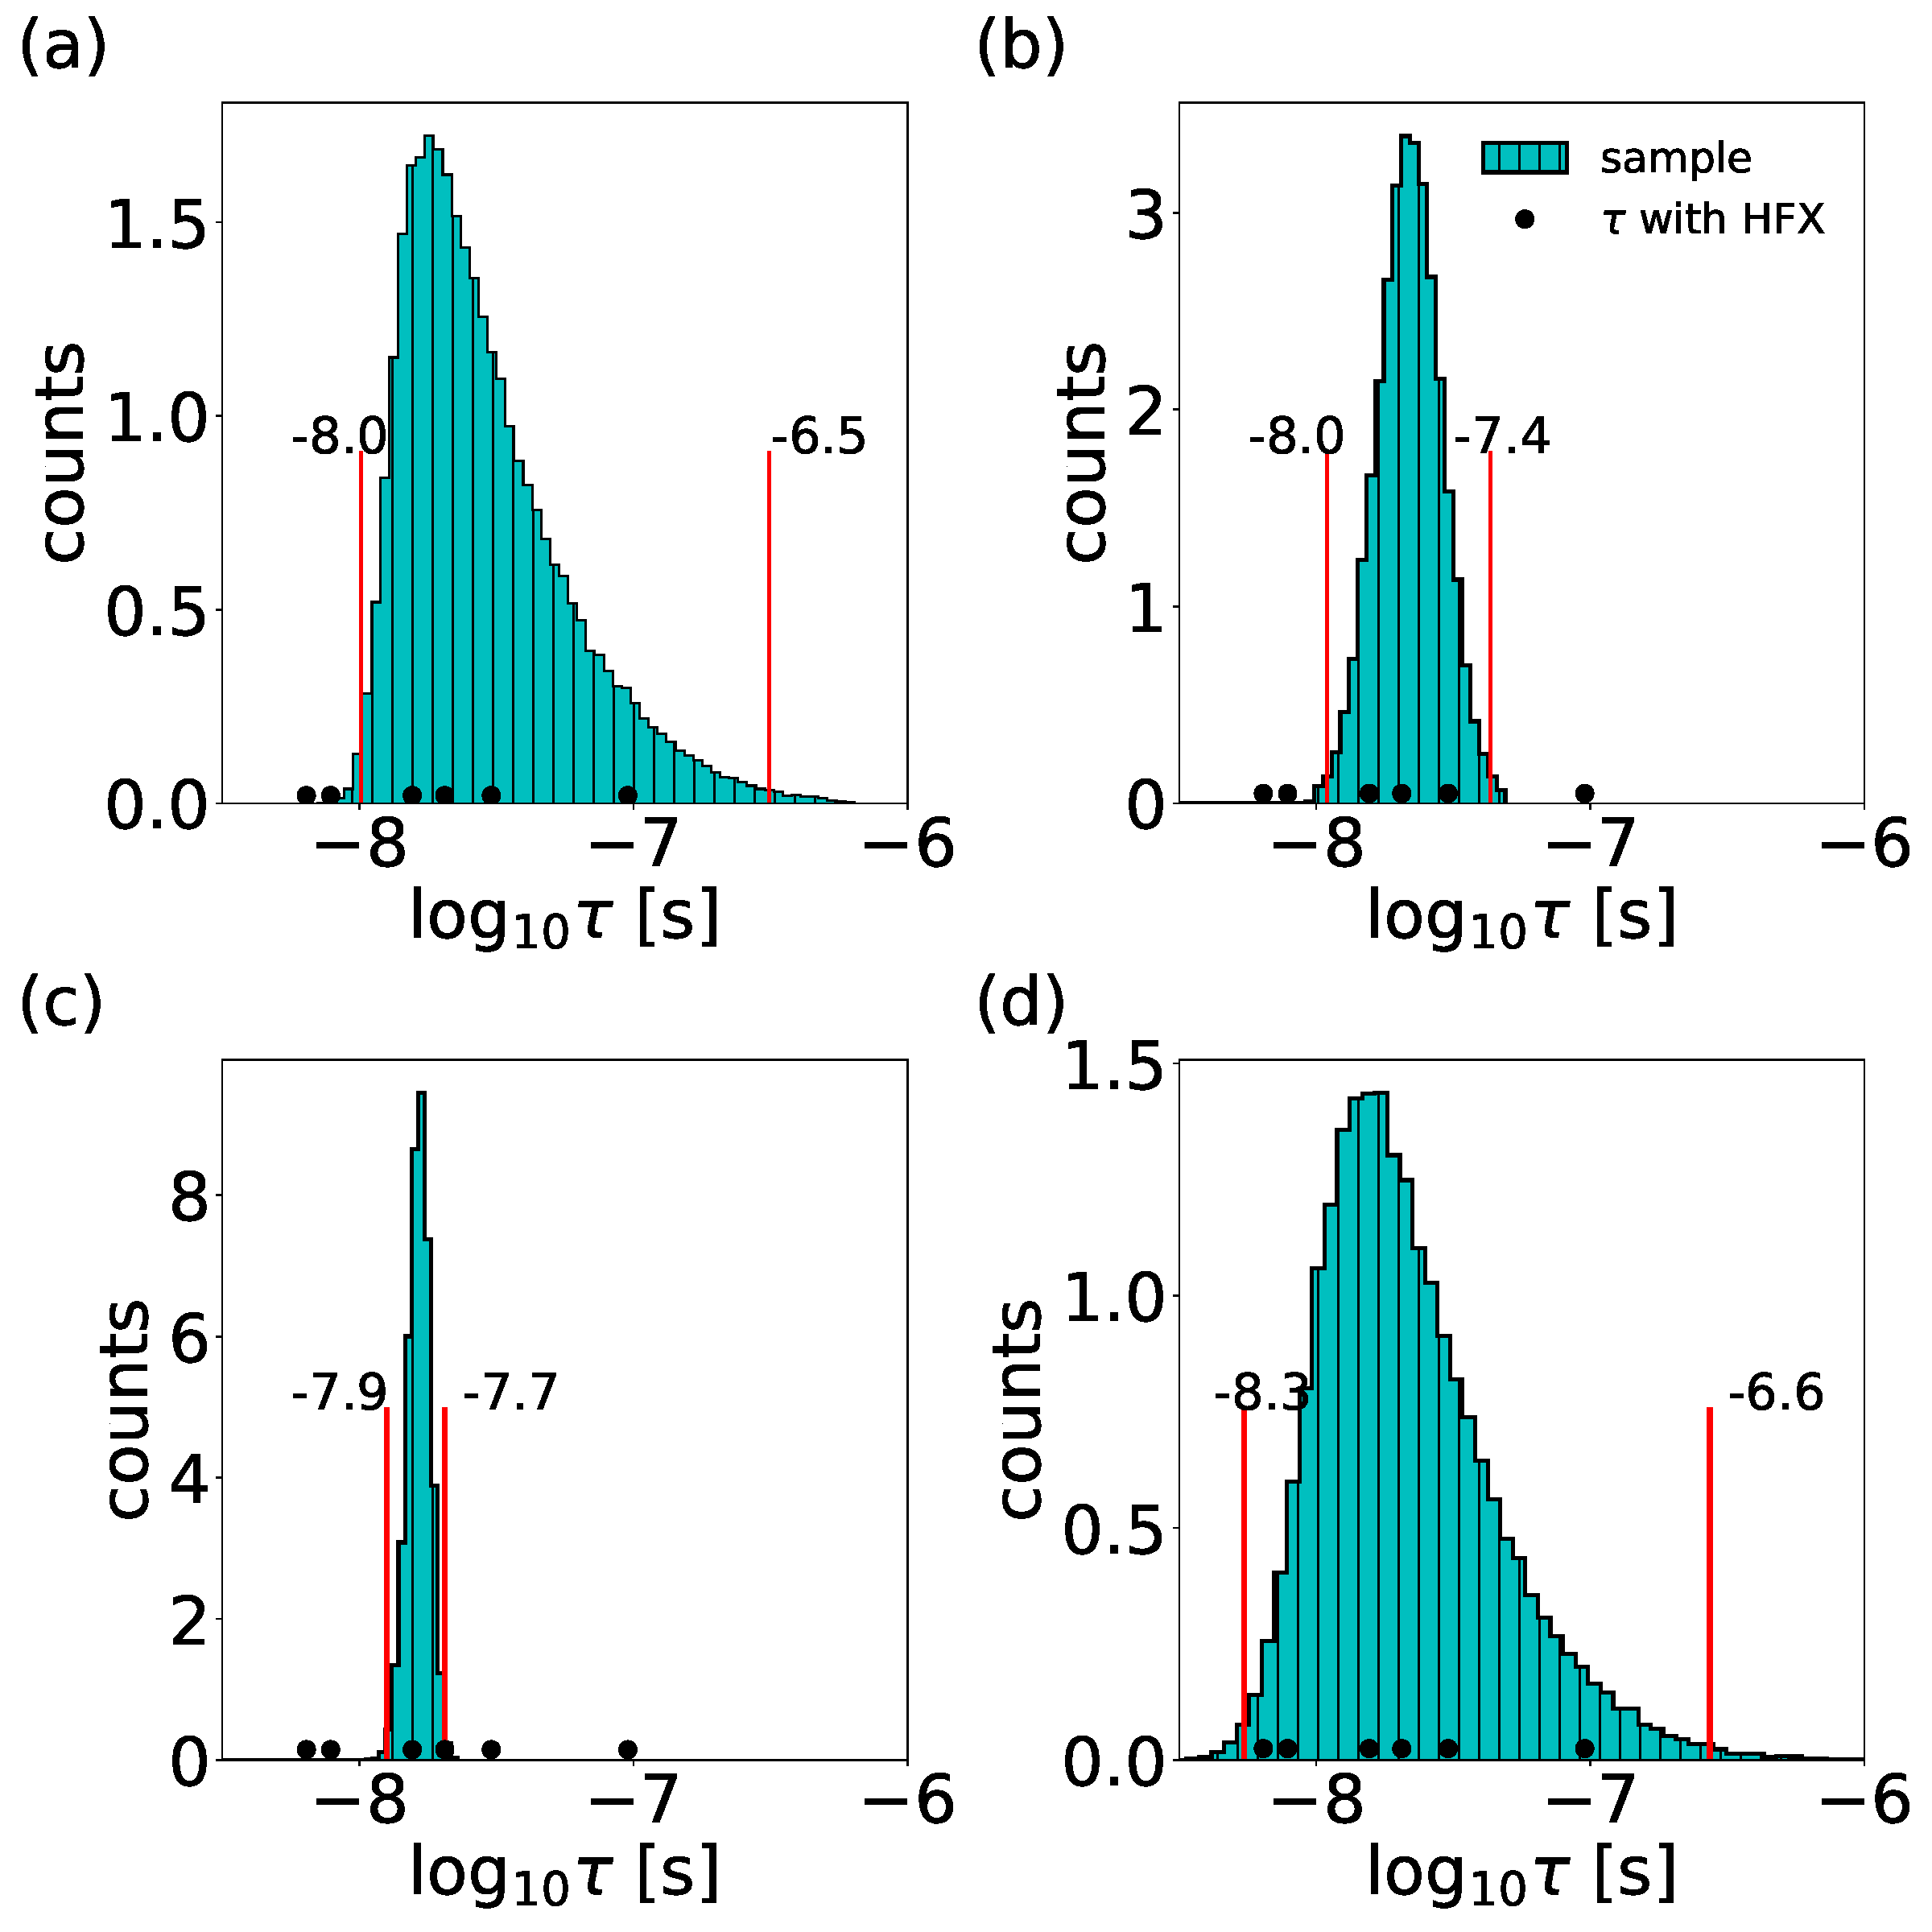
\includegraphics[width=0.45\textwidth]{figs/fig_mle_MADN_withE.pdf}
  \caption{\bjoern{TODO Zhong:}{swap panels a and b}Distribution of ToFs in the multiscale modeled MADN system.
  Monte Carlo sampling with a sample size $N_\text{MC}=50000$ is used to obtain the sampled distribution. The red vertical lines indicate the lower bound and upper bound of the 99\% confidence interval around the median.
  The black circles indicate the ToF obtained using varying HFX values.
  (a) $P(\log_{10}(\tau)|E_i \text{ uncertain})$, 
  (b) $P(\log_{10}(\tau)|\lambda \text{ uncertain})$, 
  (c) $P(\log_{10}(\tau)|J_{ij} \text{ uncertain})$, 
  (d) $P(\log_{10}(\tau)|E_i, \lambda, J_{ij} \text{ uncertain})$. }
  \label{fig:mle_MADN_withE}
\end{figure}


%The distribution that we want to obtained during the parameter control are as followed:
%\begin{enumerate}
%    \item Fixed the $\lambda$ to be $\mathbb{E}(\lambda)$, and $\log_{10}(J_{ij}^2)$ to be $\mathbb{E}(\log_{10}(J_{ij}^2))$. Then each molecule energy $E_i$ is sampled from the normal distribution $\mathcal{N}(\mathbb{E}(E_i), \mathbb{V}(E_i))$. Finally obtain and plot the histogram $N_\text{MC}$ sample of $\tau$, whose distribution is denoted as $P(\log_{10}(\tau)|E_i \text{ uncertain})$.
%    \item Fixed all $E_i$ to be $\mathbb{E}(E_i)$ and all $\log_{10}(J_{ij}^2)$ to be $\mathbb{E}(\log_{10}(J_{ij}^2))$. Then $\lambda$ is sampled from the normal distribution $\mathcal{N}(\mathbb{E}(\lambda), \mathbb{V}(\lambda))$. Finally obtain and plot the histogram  $N_\text{MC}$ sample of $\tau$, whose distribution is denoted as $P(\log_{10}(\tau)|\lambda \text{ uncertain})$. 
%    \item Fixed the $\lambda$ to be $\mathbb{E}(\lambda)$ and all $E_i$ to be $\mathbb{E}(E_i)$.     Then $J_{ij}$ is sampled from the normal distribution $\log_{10}(J_{ij}^2) \in \mathcal{N}(\mathbb{E}(\log_{10}(J_{ij}^2)), \mathbb{V}(\log_{10}(J_{ij}^2)))$. Finally obtain and plot the histogram  $N_\text{MC}$ sample of $\tau$, whose distribution is denoted as $P(\log_{10}(\tau)|J_{ij} \text{ uncertain})$.
%    \item Both $E_i$, $\lambda$ and $J_{ij}$ are sampled from their normal distribution:
    
%    $\lambda_i \in \mathcal{N}(\mathbb{E}(\lambda), \mathbb{V}(\lambda))$, 
    
%    $E_i \in \mathcal{N}(\mathbb{E}(E), \mathbb{V}(E))$, 
    
%    $\log_{10}J_{ij}^2 \in \mathcal{N}(\mathbb{E}(\log_{10}J_{ij}^2), \mathbb{V}(\log_{10}J_{ij}^2))$.
%    Then obtain and plot the histogram $N_\text{MC}$ sample of $\tau$, whose distribution is denoted as the following distribution: 
%    $P(\log_{10}(\tau)|E_i, \lambda, J_{ij} \text{ uncertain})$.
%\end{enumerate}

%The analytical forms of the distribution $P_\lambda(\log_{10}(\tau))$, $P_E(\log_{10}(\tau))$, $P_J(\log_{10}(\tau))$ and $P_\mathbf{x}(\log_{10}(\tau))$ are usually unknown. 
%To quantify the uncertainty and variability in the sample data, we calculate a $99\%$ confidence interval around the median. 
%This statistical quantity is typically nonparametric, and relies on percentiles of the data, making it robust to different types of probability mass function.

%Using the equal-tailed percentile method, its calculation involves sorting the data and determining percentiles that correspond to the desired confidence level.
%Given a dataset $\{ \tau_1, \tau_2, \dots, \tau_n \}$, the procedure can be described as follows:
%\begin{enumerate}
%  \item Sort the data in ascending order. For a confidence level $CL$, the corresponding complement 
%  $1-CL$ determines the tails of the interval. 
%  \item Find the lower bound $\tau_{\eta}$ corresponds to the $\eta$-th percentile of the dataset where $\eta = (1-CL)/2$. For a $99\%$ confidence interval, $\eta=0.05$.
%  \item Find the upper bound $\tau_{(1-\eta)}$ corresponds to the $(1-\eta)$-th percentile of the dataset.
%  \item The confidence interval around the median is $[\tau_{\eta}, \tau_{(1-\eta)}]$.
%\end{enumerate}

The four respective distributions of $\tau$ in the MADN system are shown in Fig.~\ref{fig:mle_MADN_withE} together with the indicated confidence intervals. Considering first the three distributions with single property sampling in panels (a)-(c), we find the confidence intervals for $\log_{10}(\tau)$ of $[-8.0,-7.4]$ for uncertain $\lambda$, $[-8.0,-6.5]$ for uncertain $E$, and $[-7.9,-7.7]$ for uncertain $J$, respectively. Interestingly, all three share very similar lower limits of the confidence interval, while the upper limits and the shape of the distributions differ significantly. 
\bjoern{STOP}{HERE}


The lower and upper bounds in Fig. \ref{fig:mle_MADN_withE} shows that when only the energies $E_i$ are uncertain, the $\log_{10}(\tau)$ has lower -8.0 and upper bound -6.5. This lower and upper bound is close to that of $P(\log_{10}(\tau)|E_i, \lambda, J_{ij} \text{ uncertain})$, meaning that varying the energy alone generates a $\tau$ distribution close to that when $E_i, \lambda, J_{ij}$ are uncertain. 

Figure .\ref{fig:mle_MADN_withE}(b) shows that $\log_{10}(\tau)$ has a confidence interval of -8.0 to -7.4 when $\lambda$ is varied. 
Figure \ref{fig:mle_MADN_withE}(c) show that when $J_{ij}$ is uncertain $\log_{10}(\tau)$ has a narrow confidence interval of -7.9 to -7.7, suggesting that the variation in $J_{ij}$ leads to relatively small change in $\log_{10}(\tau)$ compared to $E_i$ and $\lambda$.

%
\begin{figure}[t]
  \centering
  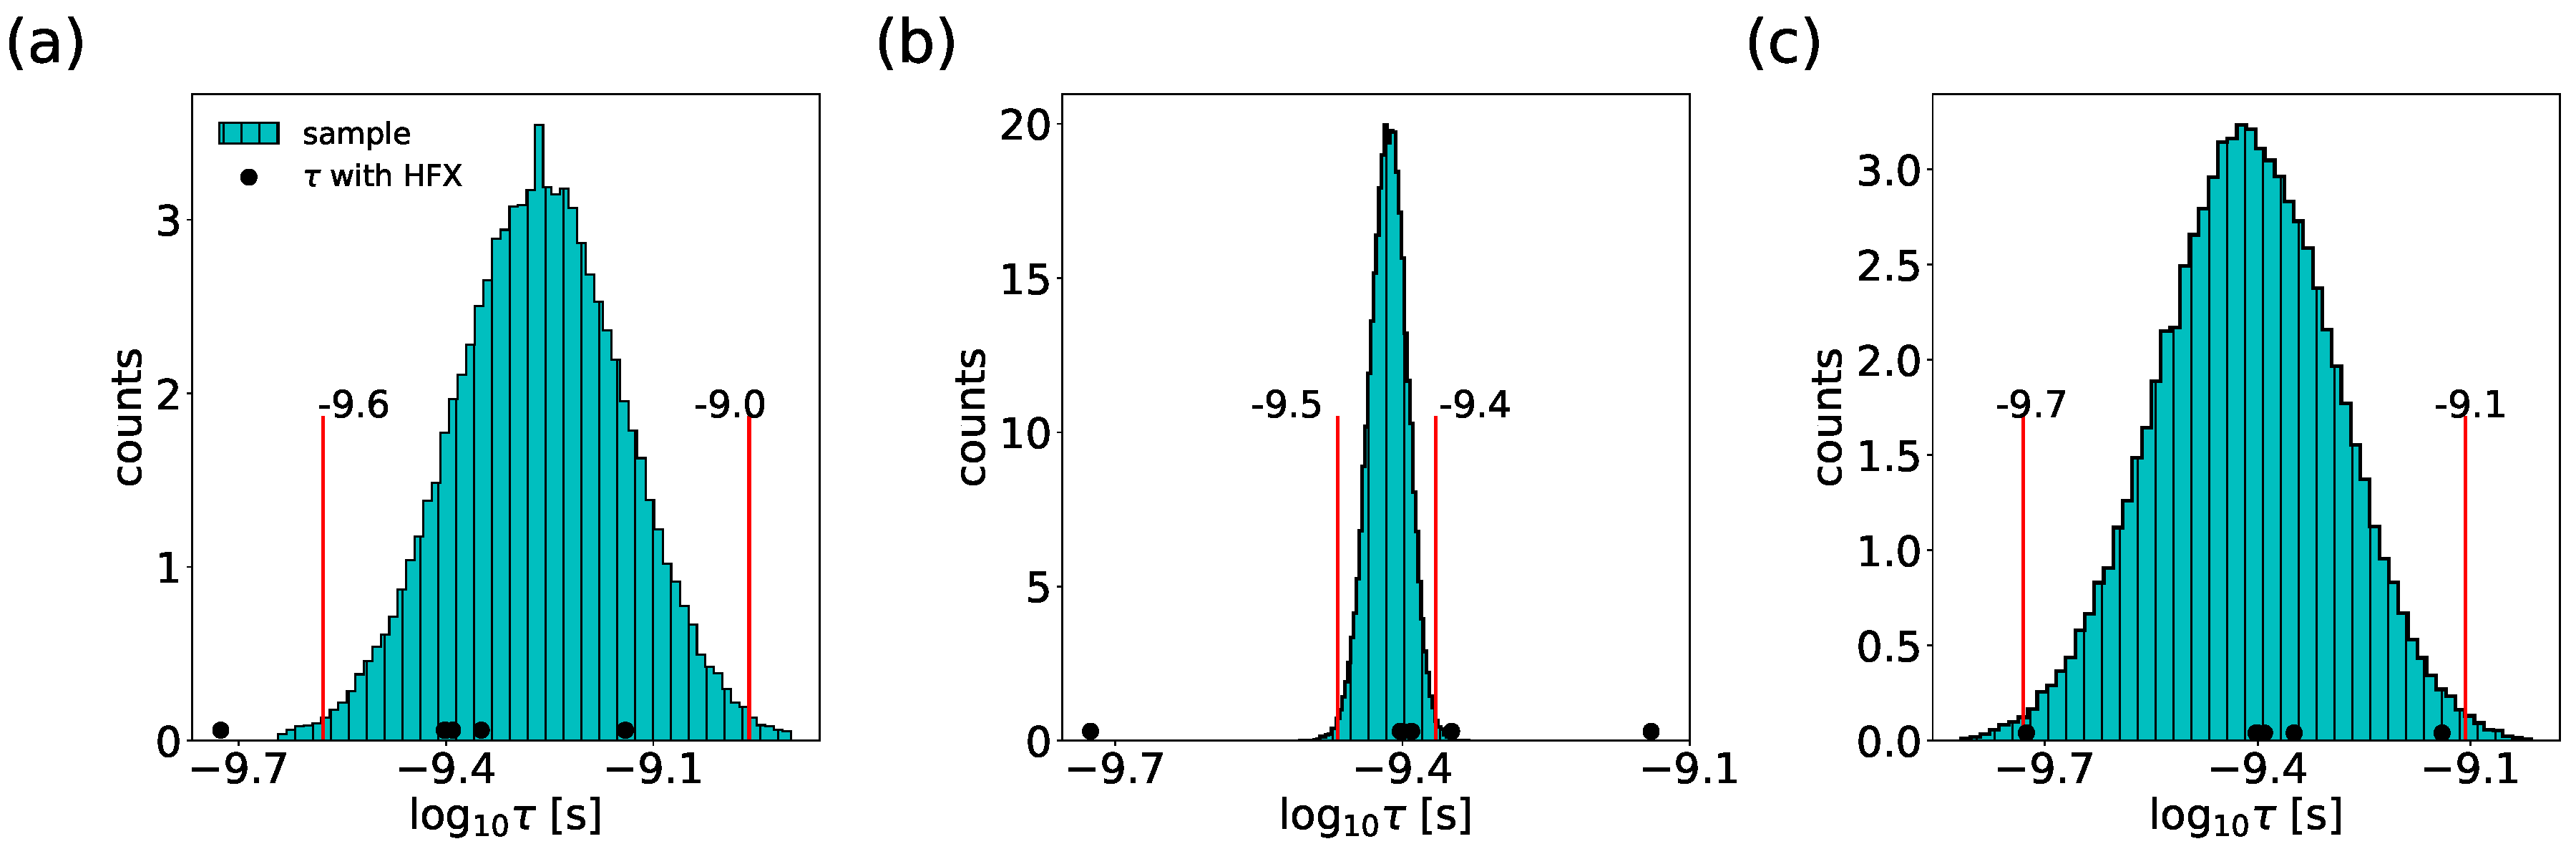
\includegraphics[width=0.45\textwidth]{figs/fig_mle_MADN_noE.pdf}
  \caption{\bjoern{TODO Zhong:}{these should also strictly be $\log_{10}(\tau/\unit[]{s})$.}Distribution of ToFs in the multiscale modeled MADN system.
  Monte Carlo sampling with a sample size $N_\text{MC}=50000$ is used to obtain the sampled distribution. The red vertical lines indicate the lower bound and upper bound of the 99\% confidence interval around the median.
  Energy disorder is not consider. 
  The black circles indicate the ToF obtained using varying HFX values.
  (a) $P(\log_{10}(\tau)|\lambda \text{ uncertain})$, 
  (b) $P(\log_{10}(\tau)|J_{ij} \text{ uncertain})$, 
  (c) $P(\log_{10}(\tau)|\lambda, J_{ij} \text{ uncertain})$. }
  \label{fig:mle_MADN_noE}
\end{figure}
%

When the energy disorder in MADN system is not considered, that is, all the MADN molecule energy are set to be equal giving $\Delta E=0$, the distribution of ToF is shown in Fig.\ref{fig:mle_MADN_noE}. 
The distribution $P(\log_{10}(\tau)|\lambda \text{ uncertain})$ has a range of confidence interval -9.6 to -9.0 resembles that of $P(\log_{10}(\tau)|\lambda, J_{ij} \text{ uncertain})$, which has a range of confidence interval -9.7 to -9.1. 



\subsection{Sobol indices}
Measuring the sensitivity of each electronic parameter to ToF is to measure each electronic parameter's contribution to the variance of ToF. 
That is, if ToF is most sensitive to one parameter, the variance in this particular parameter will contribute most to the ToF variance. 


One way of decomposing the variance of the model output into fractions attributed to input parameters is the variance-based sensitivity analysis. The local sensitive analysis is to use the partial derivative $\frac{\partial \tau}{\partial x_i}$. While the global sensitivity analysis can use Sobol's indices. Given a model of Equation \ref{eq:tau1}, to measure the parameter $x_i$'s contribution to $\tau$ including all variance caused by its interaction with other parameters $\{x_k, k \neq i \}$, the total effect Sobol's index is calculated as \cite{saltelli_variance_2010}:
\begin{equation}
    S_{T,i} = \frac{ \mathbb{E}_{\mathbf{x}_{\sim i}}[ \mathbb{V}_{x_i}(\tau|\mathbf{x}_{\sim i}) ] }{ \mathbb{V}(\tau) }
    \label{eq:STi}
\end{equation}
The details of the notation is as followed: the vector $\mathbf{x}=(x_1, x_2, \cdots, x_{N_d})$, and $\mathbf{x}_{\sim i}$ denotes the vector of all entries but $x_i$. 
$\mathbb{V}_{x_i}(\tau|\mathbf{x}_{\sim i})$ means the variance of $\tau$ given a set of $\mathbf{x}_{\sim i}$ taken over $x_i$. And $ \mathbb{E}_{\mathbf{x}_{\sim i}}[\cdot]$ denotes the mean of argument $(\cdot)$ taken over all factors but $x_i$.

%
\begin{table}[tbp]%The best place to locate the table environment is directly after its first reference in text
\caption{\label{tab:Sobol}%
Sobol indices of $\lambda$, $E$ and $\log_{10} J^2$ when ToF is calculated with energy disorder, and Sobol indices of $\lambda$ and $\log_{10} J^2$ when ToF is calculated without energy disorder.
}
\begin{ruledtabular}
  \begin{center}
    \begin{tabular}{c c c c c c c} %\hline
      &  \multicolumn{3}{c}{\bf Energy Disorder} & &\multicolumn{2}{c}{\bf no Disorder}\\\cline{2-4}  \cline{6-7}
      parameter  & $\lambda$ & $ E_i$ & $ \log_{10}(J_{ij}^2)$ && $\lambda$ & $ \log_{10}(J_{ij}^2)$ \\ \hline
      %\multicolumn{6}{c}{\bf GRW for $\mathbf{N_c=1}$}\\
   $S_T$  & 0.097 & 0.95 & 0.018 && 0.96 & 0.11 \\
    \end{tabular}
  \end{center}
\end{ruledtabular}
\end{table}
%
Then the $\lambda$ contribution to the total variance is $S_{T,i=1}$.
The energy contribution to the total variance is $S_{T,E} = \sum\limits_{i=1}^{N+1} S_{T,i}$ where $N=1000$ is the number of energy parameter, and the coupling element contribution due to variation in $\log_{10}(J_{ij}^2)$ to the total variance is $S_{T,J}=\sum\limits_{i=N+2}^{N_d} S_{T,i}$. 
Using the quasi Monte Carlo method\cite{sobol_global_2001} with a sample size $N_\text{QMC}=1000$ to calculate $S_{T,i}$, the results are shown in the table \ref{tab:Sobol}.

From table \ref{tab:Sobol} one can see that most of the total variance can be attributed to the energy $E$. In contrast to $E$, the uncertainty in $\lambda$ and $\log_{10} J^2$ contributes much less compared to $E$, this is consistent to the Fig.\ref{fig:mle_MADN_withE}, where the distribution in Fig.\ref{fig:mle_MADN_withE}(d) resembles the distribution in Fig.\ref{fig:mle_MADN_withE}(a).
And Fig.\ref{fig:mle_MADN_withE}(c) shows that the uncertainty in $\log_{10}(J^2)$ only leads to small variances.
When there is no energy disorder, the variance in $\lambda$ has the most contribution to the total variance as shown in Table \ref{tab:Sobol}.

%%%%%%%%%%%%%%%%%%%%%%%%%%%%%%%%%%%%%%%%%%%%%%%%%%%%%%%%%%%%%%%%%%%
%
%\begin{figure}
%  \centering
%  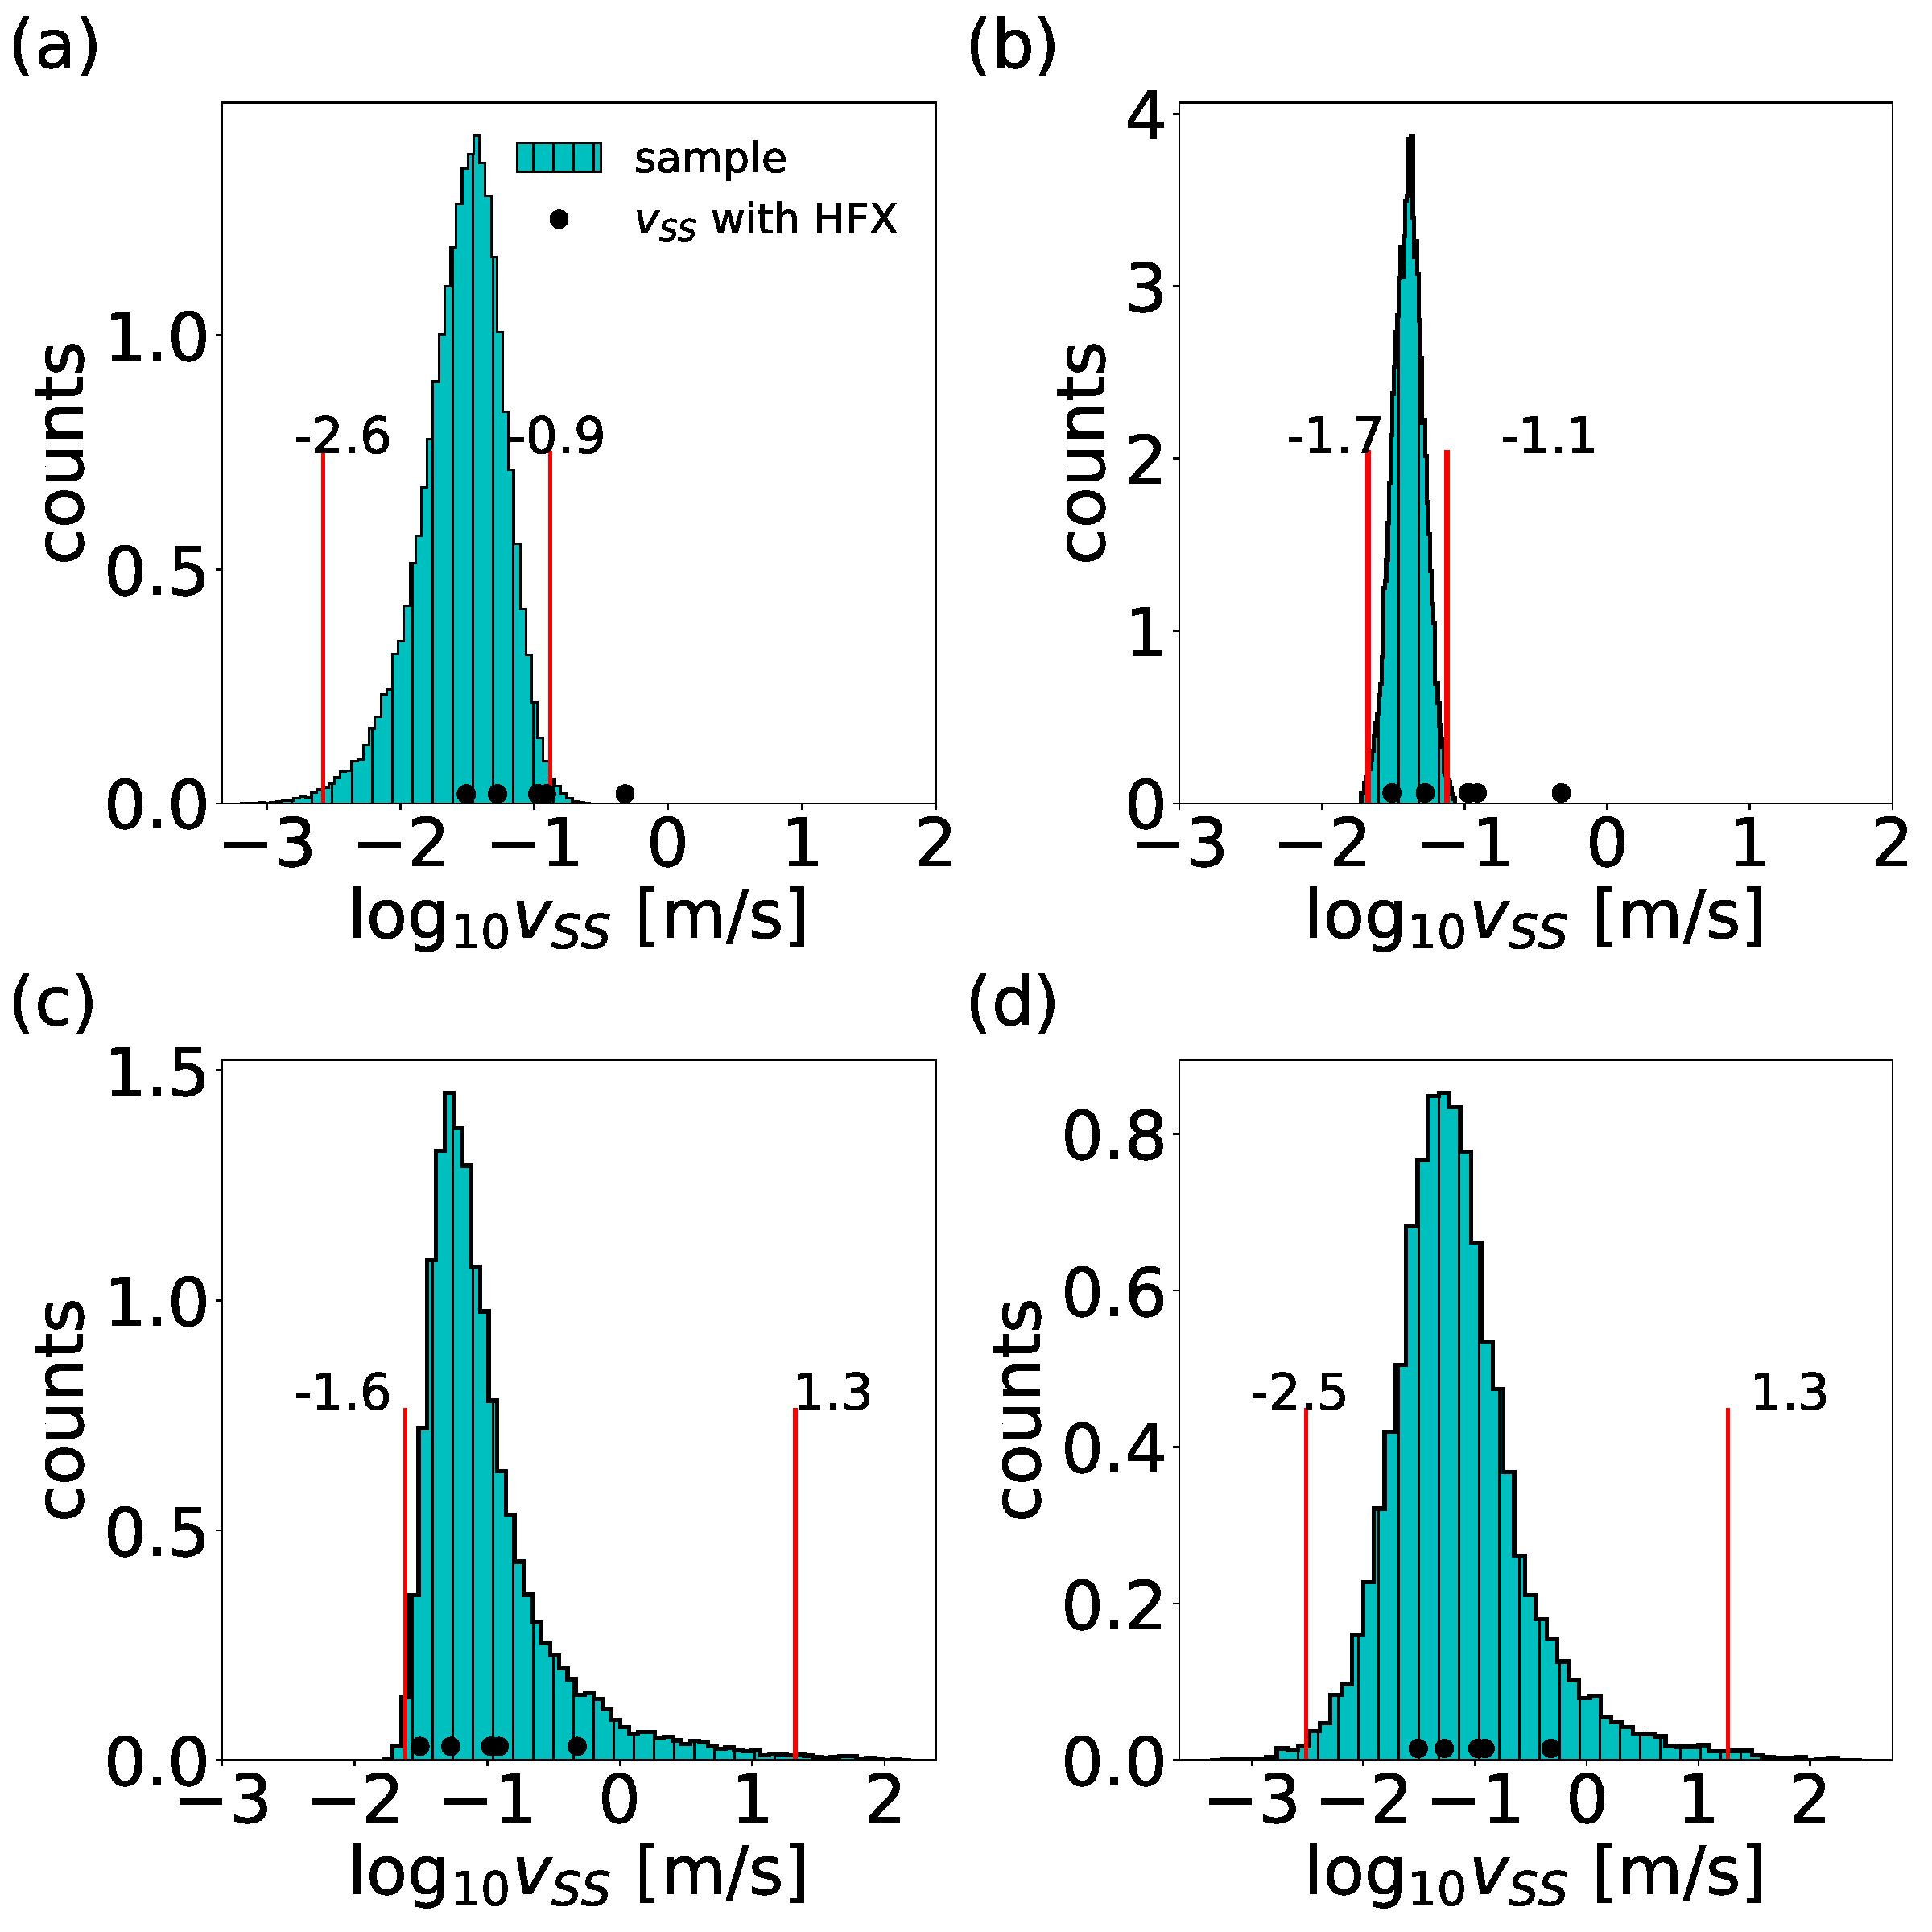
\includegraphics[width=0.45\textwidth]{figs/fig_mle_MADN_withE_SS.pdf}
%  \caption{Distribution of steady state velocity $v_\text{SS}$ in the multiscale modeled MADN.
%  Monte Carlo sampling with a sample size $N_\text{MC}=50000$ is used to obtain the sampled distribution.
%  The red vertical lines indicate the lower bound and upper bound of the 99\% confidence interval around the median.
%  The black circles indicate the $v_\text{SS}$ obtained using varying HFX values.
%  (a) $P(\log_{10}(v_\text{SS})|E_i \text{ uncertain})$, 
%  (b) $P(\log_{10}(v_\text{SS})|\lambda \text{ uncertain})$, 
%  (c) $P(\log_{10}(v_\text{SS})|J_{ij} \text{ uncertain})$, 
%  (d) $P(\log_{10}(v_\text{SS})|E_i, \lambda, J_{ij} \text{ uncertain})$. }
%  \label{fig:mle_MADN_withE_SS}
%\end{figure}
%
%
%\begin{figure}
%  \centering
%  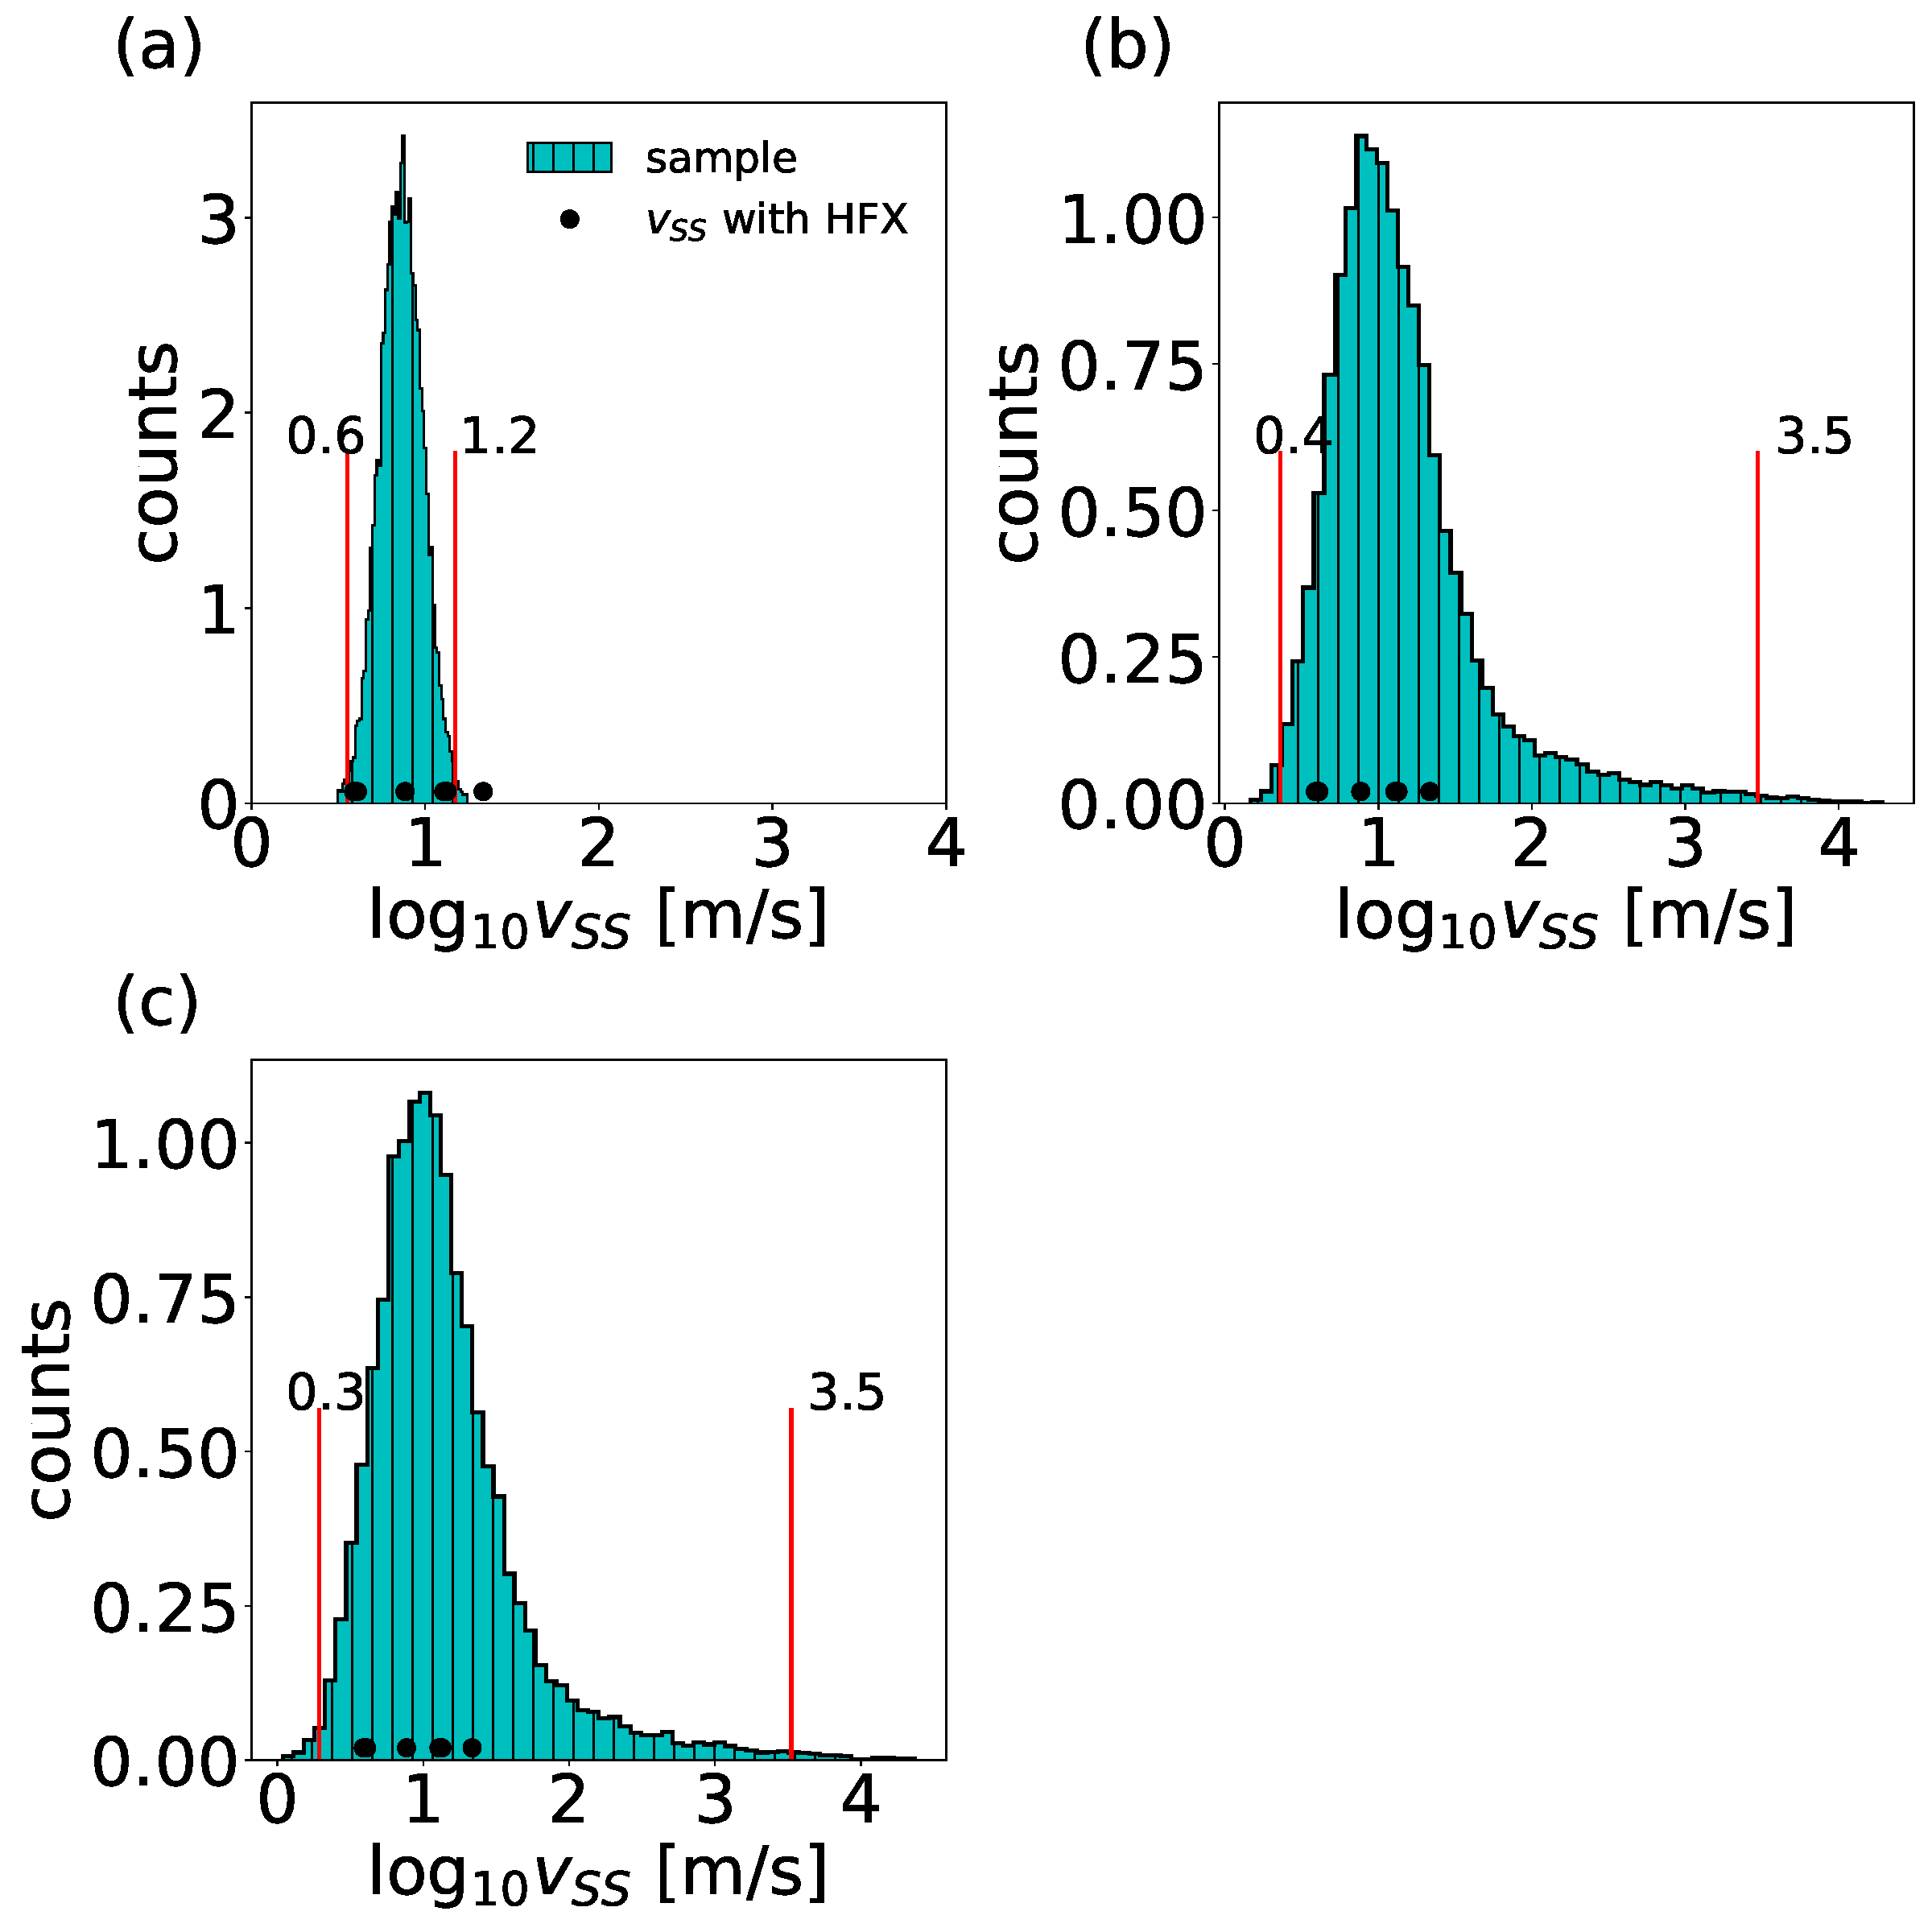
\includegraphics[width=0.45\textwidth]{figs/fig_mle_MADN_noE_SS.pdf}
%  \caption{Distribution of steady state velocity $v_\text{SS}$ in the multiscale modeled MADN. All molecule energies are set to be zero.  
%  Monte Carlo sampling with a sample size $N_\text{MC}=50000$ is used to obtain the sampled distribution.
%  The red vertical lines indicate the lower bound and upper bound of the 99\% confidence interval around the median.
%  The black circles indicate the $v_\text{SS}$ obtained using varying HFX values.
%  (a) $P(\log_{10}(v_\text{SS})|\lambda \text{ uncertain})$, 
%  (b) $P(\log_{10}(v_\text{SS})|J_{ij} \text{ uncertain})$, 
%  (c) $P(\log_{10}(v_\text{SS})|\lambda, J_{ij} \text{ uncertain})$.  }
%  \label{fig:mle_MADN_noE_SS}
%\end{figure}


%\section{Distribution of Steady State Velocity}

%The distribution of steady state velocity of MADN is shown as Fig.\ref{fig:mle_MADN_withE_SS} and \ref{fig:mle_MADN_noE_SS}. 
%From the confidence interval, $P(\log_{10}(v_\text{SS})|E_i \text{ uncertain})$ has a range of -2.6 to -0.9, and the confidence interval $P(\log_{10}(v_\text{SS})|\lambda \text{ uncertain})$ has a range from -1.7 to -1.1. The width of those confidence intervals is very close to the confidence interval of distributions $P(\log_{10}(\tau)|E_i \text{ uncertain})$ and $P(\log_{10}(\tau)|\lambda \text{ uncertain})$, respectively.
%However, $P(\log_{10}(v_\text{SS})|J_{ij} \text{ uncertain})$ has a range from -1.6 to 1.3, spanning 3 orders of magnitude. This is  much larger than $P(\log_{10}(\tau)|J_{ij} \text{ uncertain})$ as shown in Fig .\ref{fig:mle_MADN_withE}.  
%The large confidence interval in $P(\log_{10}(v_\text{SS})|J_{ij} \text{ uncertain})$ shows that $v_{ss}$ is very sensitive to the change in $J_{ij}$. Combining all the uncertainty effects in $E_i, \lambda, J_{ij}$, the confidence interval of $P(\log_{10}(v_\text{SS})|E_i, \lambda, J_{ij} \text{ uncertain})$ is from -2.5 to 1.3, covering 4 orders of magnitude.  

%When energy disorder is not considered, the $v_\text{SS}$ distribution $P(\log_{10}(v_\text{SS})|\lambda, J_{ij} \text{ uncertain})$ has a confidence interval from 0.3 to 3.5, spanning 3 orders of magnitude. This interval is close to the range of $P(\log_{10}(v_\text{SS})|J_{ij} \text{ uncertain})$ when only $J_{ij}$ is uncertain. 
%In contrast, the interval of $P(\log_{10}(v_\text{SS})|\lambda \text{ uncertain})$ is from 0.6 to 1.2, whose width is much smaller than that of $P(\log_{10}(v_\text{SS})|J_{ij} \text{ uncertain})$.

%These result suggests that compared to the ToF $\tau$, the quantity $v_\text{SS}$ is significantly affected by uncertainties in $J_{ij}$, so $v_\text{SS}$ is less robust when the parameters $E_i, \lambda, J_{ij}$ contains uncertainty at the same time. 
%In the next section, the Poole–Frenkel behavior, that is the dependence of charge mobility on the electric field will be study using the ToF setting. 
%%%%%%%%%%%%%%%%%%%%%%%%%%%%%%%%%%%%%%%%%%%%%%%%%%%%%%%%%%%%%%%%%%%%%%%%%%

\section{Charge mobility and PF Behavior}

In this section, we want to study the dependence of drift mobility on the HFX. The charge mobility is calculated as:
\begin{equation}
    \mu = \frac{\vec{v} \vec{F} }{ |\vec{F}|^2}
    \label{eq:mu}
\end{equation}
To consider the charge dynamics along X, Y and Z axis in the ToF setting, the ToF is calculated with different settings of \textit{Source}-\textit{Sink} and $\vec{F}$ combinations.

\begin{itemize}
    \item Setting the molecules with $r^x < \min(r^x)+0.5$ as \textit{Source}, and the molecules with $r^x > \max(r^x)-0.5$ as \textit{Sink}, and $\vec{F}^T = (F,0,0)$, denote the calculated the ToF as $\tau_\text{Xmin}$, and the mobility is as $\mu_\text{Xmin} = \frac{L_x }{\tau_\text{Xmin} |\vec{F}|}$.  
    \item Setting the molecules with $r^x > \max(r^x)-0.5$ as \textit{Source}, and the molecules with $r^x < \min(r^x)+0.5$ as \textit{Sink}, and $\vec{F}^T = (-F,0,0)$, denote the calculated the ToF as $\tau_\text{Xmax}$, and the mobility is as $\mu_\text{Xmax} = \frac{L_x }{\tau_\text{Xmax} |\vec{F}|}$.  
    \item Setting the molecules with $r^y < \min(r^y)+0.5$ as \textit{Source}, and the molecules with $r^y > \max(r^y)-0.5$ as \textit{Sink}, and $\vec{F}^T = (0,F,0)$, denote the calculated the ToF as $\tau_\text{Ymin}$, and the mobility is as $\mu_\text{Ymin} = \frac{L_y }{\tau_\text{Ymin} |\vec{F}|}$. 
    \item Setting the molecules with $r^y > \max(r^y)-0.5$ as \textit{Source}, and the molecules with $r^y > \max(r^y)-0.5$ as \textit{Sink}, and $\vec{F}^T = (0,-F,0)$, denote the calculated the ToF as $\tau_\text{Ymax}$, and the mobility is as $\mu_\text{Ymax} = \frac{L_y }{\tau_\text{Ymax} |\vec{F}|}$. 
    \item Setting the molecules with $r^z < \min(r^z)+0.5$ as \textit{Source}, and the molecules with $r^z > \max(r^z)-0.5$ as \textit{Sink}, and $\vec{F}^T = (0,0,F)$, denote the calculated the ToF as $\tau_\text{Zmin}$, and the mobility is as $\mu_\text{Zmin} = \frac{L_z }{\tau_\text{Zmin} |\vec{F}|}$. 
    \item Setting the molecules with $r^z > \max(r^z)-0.5$ as \textit{Source}, and the molecules with $r^z > \min(r^z)+0.5$ as \textit{Sink}, and $\vec{F}^T = (0,0,-F)$, denote the calculated the ToF as $\tau_\text{Zmax}$, and the mobility is as $\mu_\text{Zmax} = \frac{L_z }{\tau_\text{Zmax} |\vec{F}|}$. 
\end{itemize}
Finally the ToF drift mobility is calculated as:
\begin{equation}
    \mu_\text{PF} = \frac{1}{6} (\mu_\text{Xmin}+\mu_\text{Xmax}+\mu_\text{Ymin}+\mu_\text{Ymax}+\mu_\text{Zmin}+\mu_\text{Zmax})
\end{equation}

When the $\lambda, E_i, J_{ij}$ are uncertain and sampled from the normal distribution, the distributions of charge mobility obtained from MC sample under specific electric field are shown in Fig.\ref{fig:fig_mle_withE_mu2_ave}.
%
\begin{figure}
    \centering
    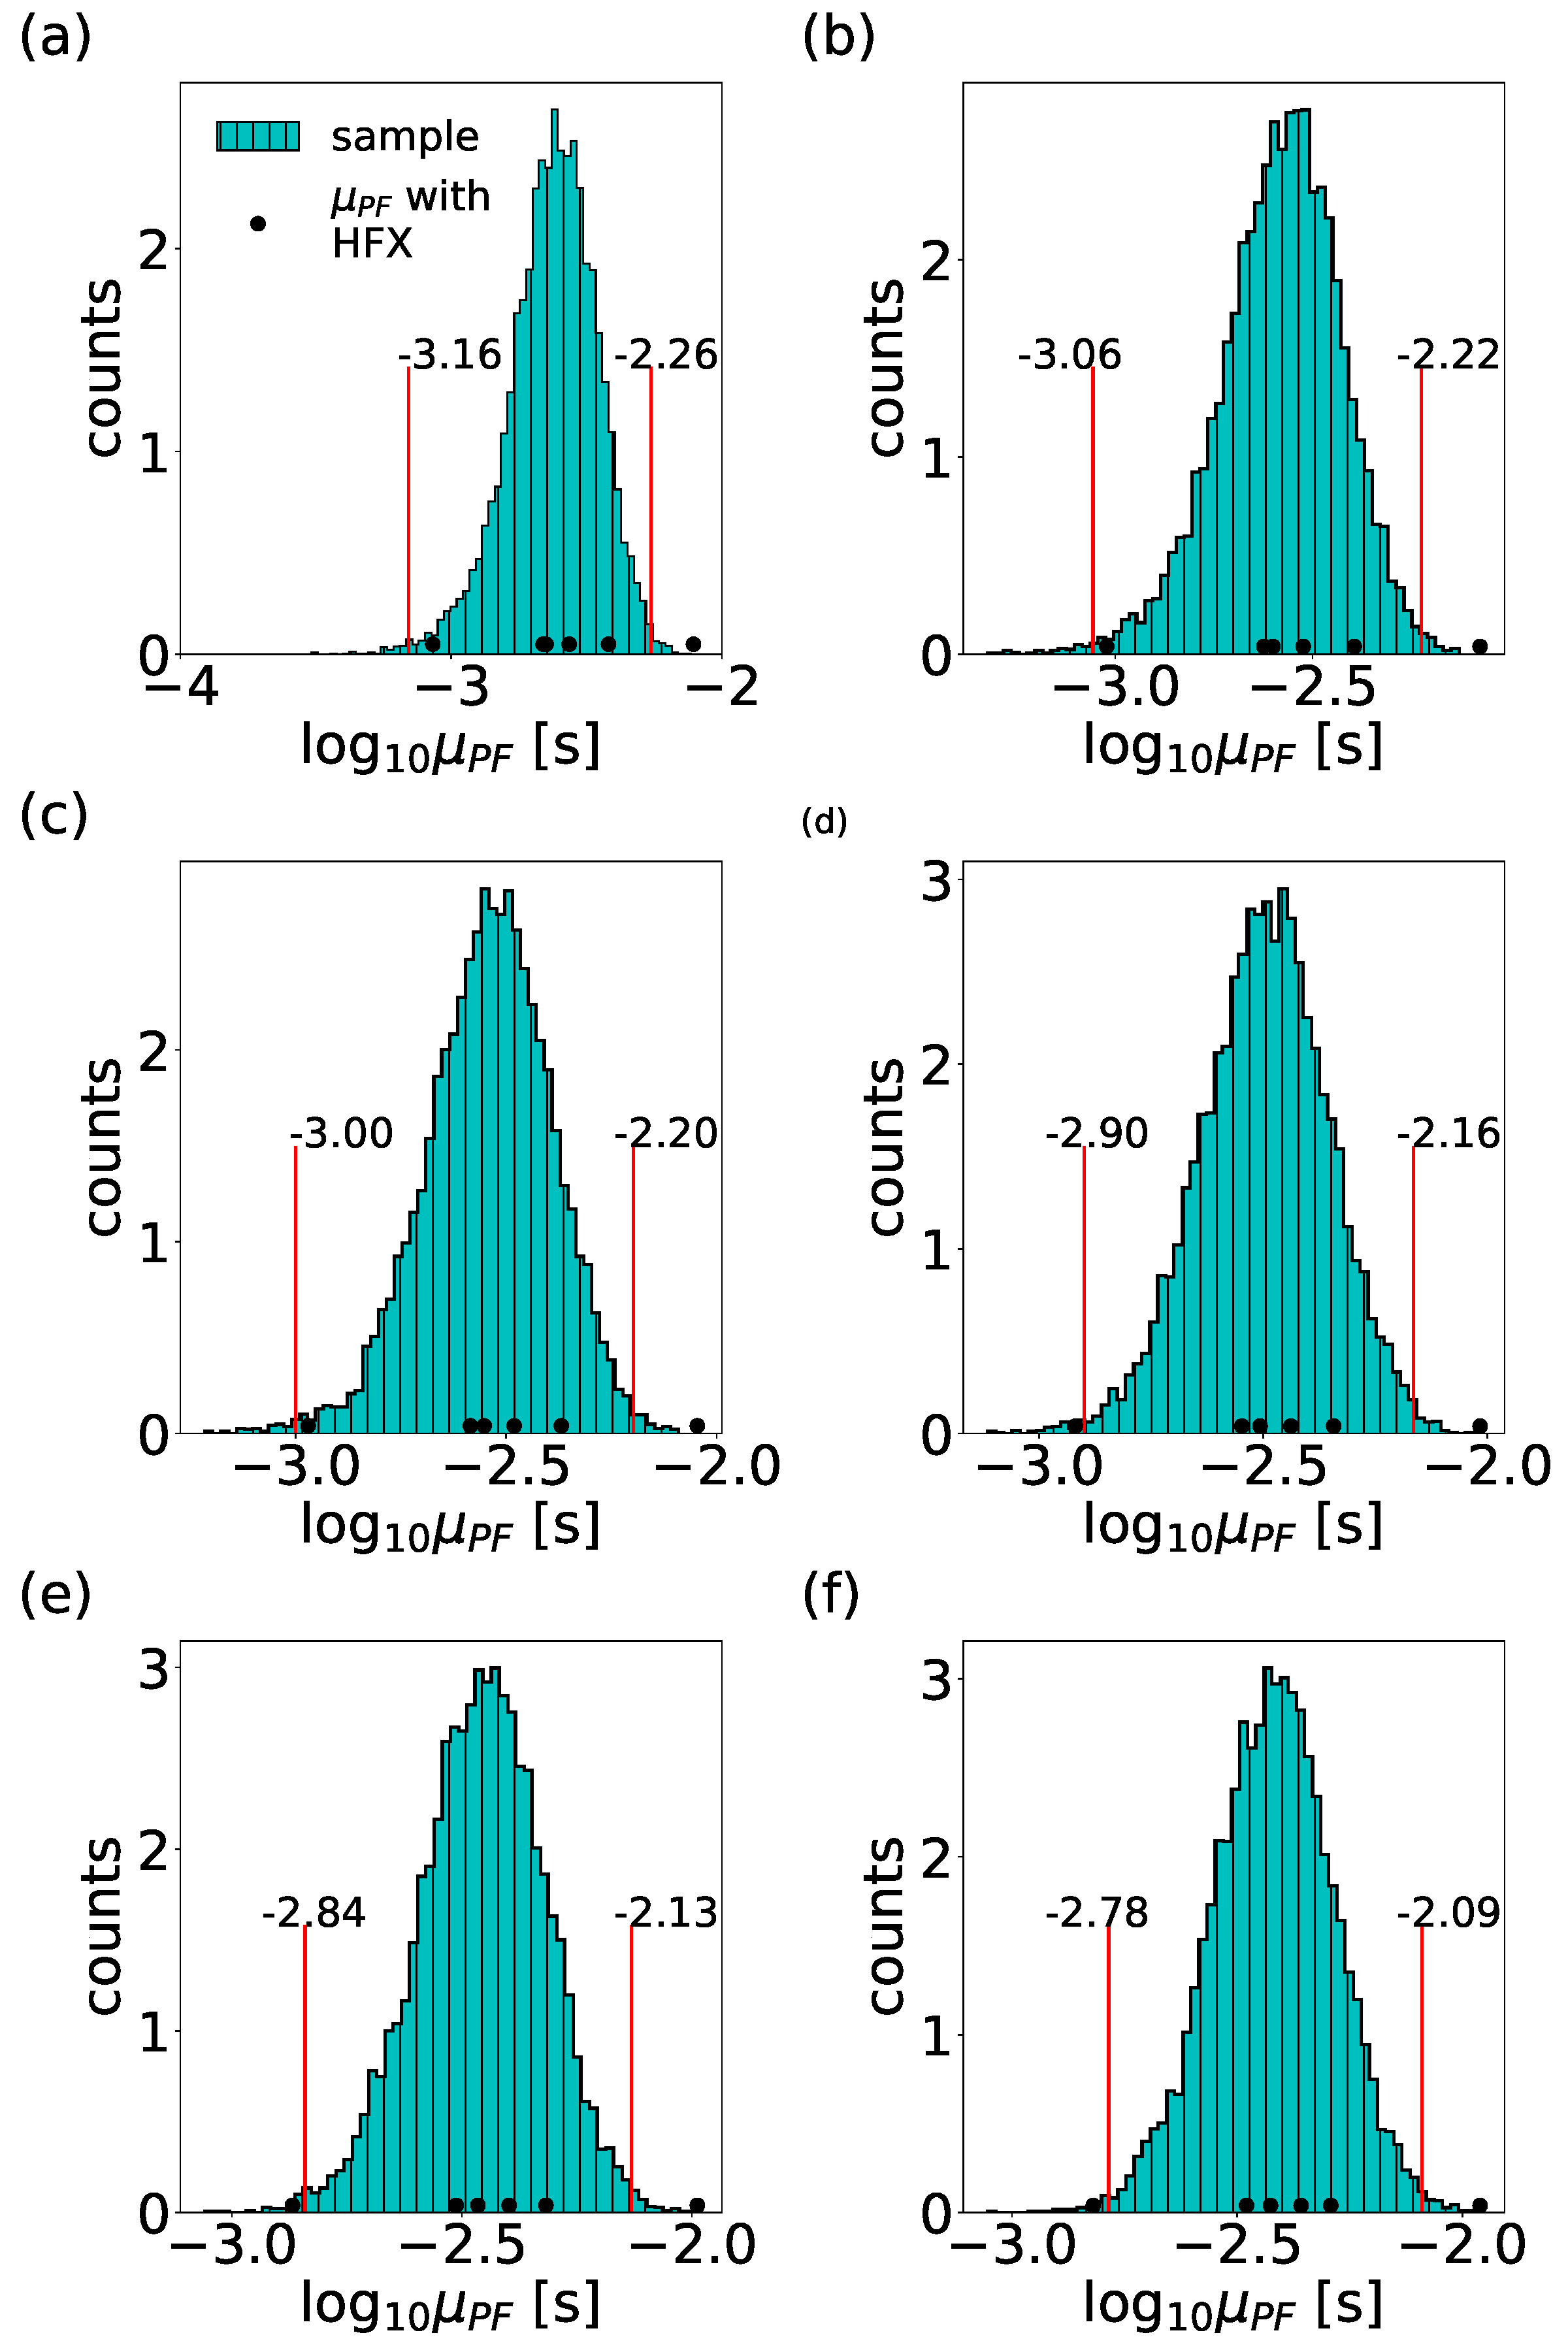
\includegraphics[width=0.45\textwidth]{figs/fig_mle_withE_mu2_ave.pdf}
    \caption{\bjoern{TODO Zhong:}{these should also strictly be $\log_{10}(\mu/(\unit[]{cm^2(Vs)^{-1}}))$; there should be no PF label at $\mu$.} Distribution of $\mu_\text{PF}$ in the multiscale modeled MADN system.
    Monte Carlo sampling with a sample size $N_\text{MC}=10000$ is used to obtain the sampled distribution. The red vertical lines indicate the lower bound and upper bound of the 99\% confidence interval around the median. (a) $|\vec{F}|=4 \cdot 10^7 \unit{V/m}$, (b) $|\vec{F}|=5 \cdot 10^7 \unit{V/m}$, (c) $|\vec{F}|=6 \cdot 10^7 \unit{V/m}$, (d) $|\vec{F}|=7 \cdot 10^7 \unit{V/m}$, (e) $|\vec{F}|=8 \cdot 10^7 \unit{V/m}$, (f) $|\vec{F}|=9 \cdot 10^7 \unit{V/m}$.}
    \label{fig:fig_mle_withE_mu2_ave}
\end{figure}
%

When the $\lambda, E_i, J_{ij}$ are uncertain and sampled from the normal distribution, the distributions of charge mobility obtained from MC sample under specific electric field are shown in Fig. \ref{fig:fig_mle_withE_mu2_ave}. The ToF depends on the electric field through the Marcus rate. As the electric increase from $|\vec{F}|=4 \cdot 10^7 \unit{V/m}$
$|\vec{F}|=9 \cdot 10^7 \unit{V/m}$, the
range of the 90\% confidence interval where $\log_{10} \mu_\text{PF}$ lies
estimated from the MC sample decrease from 0.90 to 0.69.
So the electric field results in a narrower range of $\mu_\text{PF}$ distribution.
Due to this reason, the $\mu_\text{PF}$ calculated from $\alpha=0$ is not in the 99\% confidence interval around the median of the MC sampled data, although the zero-field ToF of $\alpha=0$ is contained in the according 99\% confidence interval, as shown in Fig. \ref{fig:mle_MADN_withE}(d).

The ToF depends on the electric field through the Marcus rate. 
Poole and Frenkel \cite{frenkel_prebreakdown_1938} predicted the electric-field dependence of charge mobility as $\mu_\text{PF}(F)=\mu_0 \exp (\beta \sqrt{|\vec{F}|})$.
So it is common to plot the mobility $\mu_\text{PF}$ against $\sqrt{|\vec{F}|}$ in a so-called Poole-Frenkel plot.
which is shown in Fig. \ref{fig:PF_plot_ave} for specifie HFX values. The 99\% confidence interval obtained via MC sampled in shown in the green shadow. 
This interval suggests that if the uncertainties from the parameters are represented by the maximum likelihood distribution, the Poole–Frenkel plot from $\alpha=0$ has less 1\% chance to happen and thus is very likely. 
%
\begin{figure}[tbp]
    \centering
    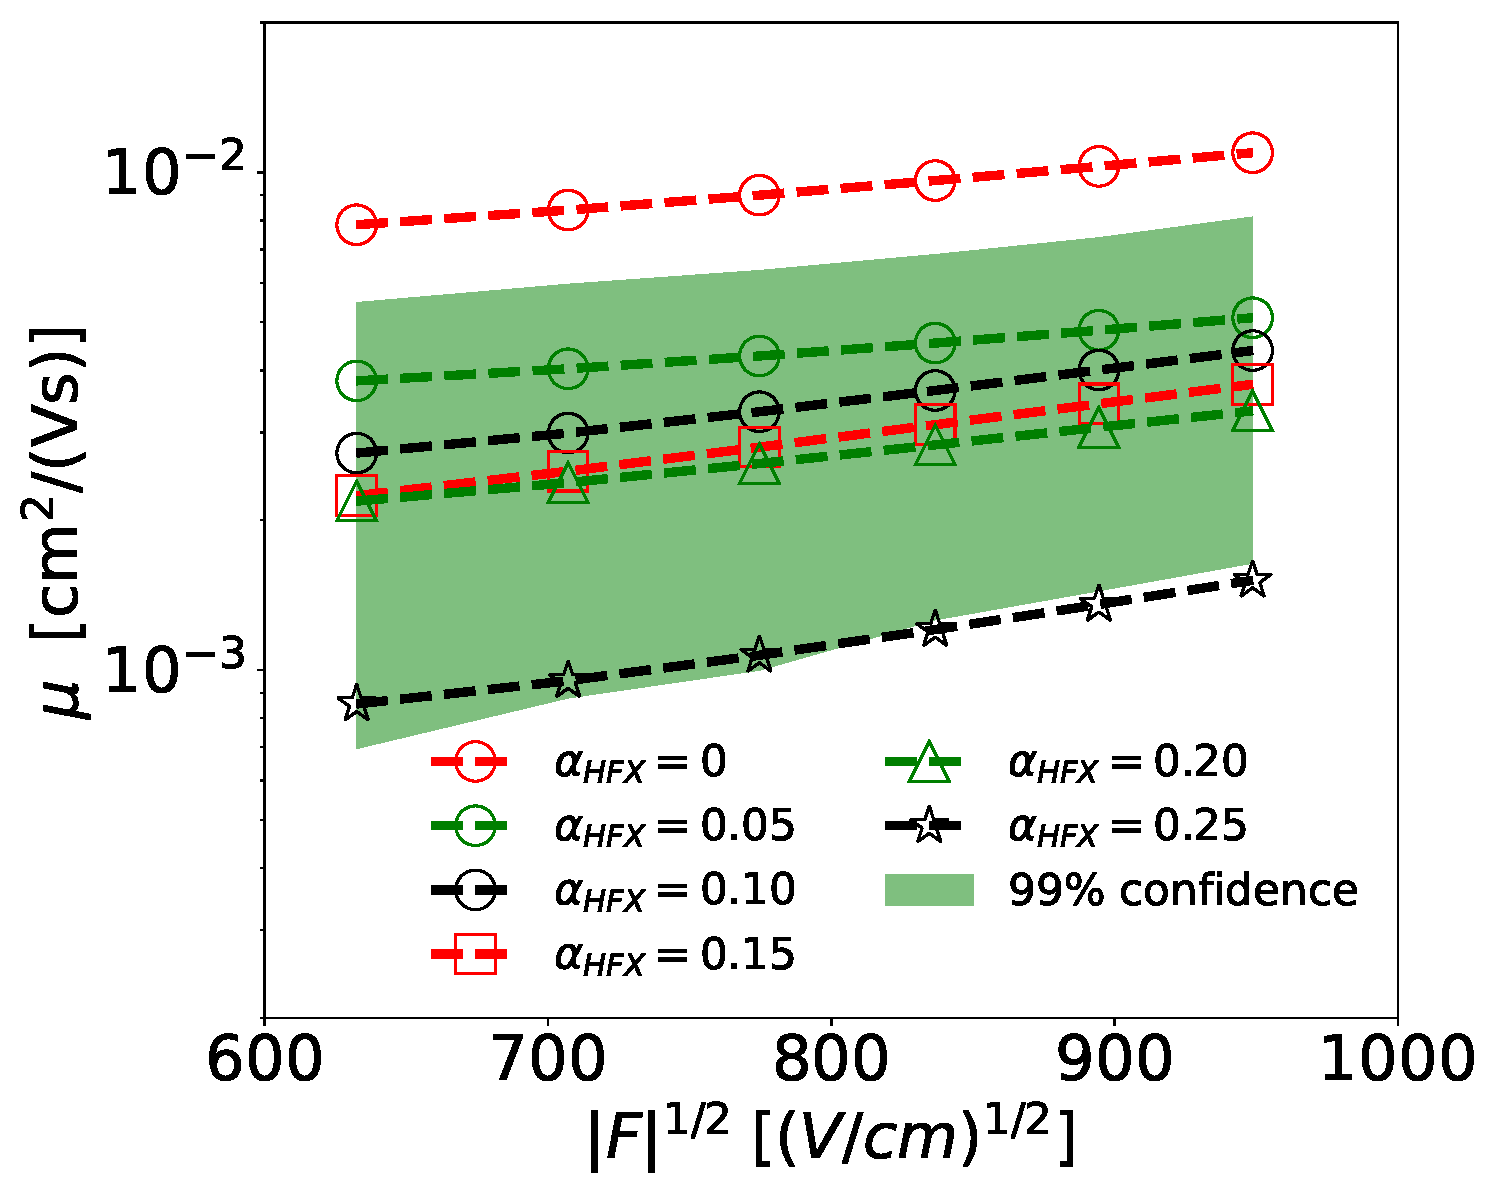
\includegraphics[width=0.45\textwidth]{figs/fig_PF_plot_ave.pdf}
    \caption{\bjoern{TODO Zhong:}{remove PF label; avoid the large white space at the right; make data plot symbols a little bigger and lines a little thicker.}Electric-field dependence of the mobility $\mu$ in the multiscale modeled MADN system. The dash lines are Poole–Frenkel plots obtained with specific HFX value, and the green shadow indicates the 99\% confidence interval estimated from the MC sampling with a sample size of $N_\text{MC}=10000$.}
    \label{fig:PF_plot_ave}
\end{figure}

%
\begin{table}[tbp]%The best place to locate the table environment is directly after its first reference in text
  \caption{\label{tab:PF_parameter}%
  Poole-Frenkel parameters $\mu_0$ (in $\unit[]{cm^2/(Vs)}$) and $\beta$ (in $\unit[]{\sqrt{cm/V}}$) of the multiscale modeled MADN, calculated by the six different HFX values. 
  }
  \begin{ruledtabular}
    \begin{tabular}{c c c c c}
    $\alpha$ & & $\mu_0$  & & $\beta$ \\
      \hline
    0 & & $4.0 \cdot 10^{-3}$ & & $1.0 \cdot 10^{-3}$ \\
    0.05 & & $2.1 \cdot 10^{-3}$ & & $9.3 \cdot 10^{-4}$ \\
    0.10 & & $1.0 \cdot 10^{-3}$ & & $1.5 \cdot 10^{-3}$ \\
    0.15 & & $8.0 \cdot 10^{-4}$ & & $1.6 \cdot 10^{-3}$ \\
    0.20 & & $9.3 \cdot 10^{-4}$ & & $1.3 \cdot 10^{-3}$ \\
    0.20 & & $2.6 \cdot 10^{-4}$ & & $1.8 \cdot 10^{-3}$ \\
      \end{tabular}
  \end{ruledtabular}
  \end{table}
%  
The extracted Poole–Frenkel paratermeter calculated from the six $\alpha$ values are summarized in Table \ref{tab:PF_parameter}. 
Excluding the data of $\alpha=0$, the extracted zero-field mobility $\mu_0$ has a range from $2.6 \cdot 10^{-4}$ to $2.1 \cdot 10^{-3}$, and the field effect constant $\beta$ range from $9.3 \cdot 10^{-4}$ to $1.8 \cdot 10^{-3}$.
So $\beta$ is less sensitive to the multiscale model parameter $\alpha$ compared the zero-field mobility.
%%%%%%%%%%%%%%%%%%%%%%%%%%%%%%%%%%%%%%%%%%%%%%%%%%%%%%%%%%%%%%%%%%%%
\section{Conclusion}
The uncertainty effect from the exchange-correlation functional of the DFT on the multiscale model of OSC is studied. By choosing different HFX, the calculated values of some electronic structures remain very similar,
such as the reorganization energy $\lambda$, molecular energy $E_i$ and the majority of the coupling elements  $J_{ij}$. While a few small-value coupling elements $J_{ij}$ show large different in calculated values when different HFX is used. Those uncertainties propagate to the output of the multiscale model, resulting in a range of QoI which has a maximum about 15 times of its minimum. These findings high-
light the importance of selecting appropriate functionals to ensure model robustness. Also indicated is that for multiscale model charge mobility, when the values have difference is approximately 10\%, we should interpret the results with caution and refrain from concluding that they represent fundamentally different phenomena.

Assuming the maximum amount of uncertainty from the calculated electronic structure parameters using the six HFX, the 99\% confidence level of the ToFs around the median are estimated. The Sobol indexes show that the molecular energy has the most contribution to the total variance, followed by the reorganization energy and coupling elements. Our results also shows that due to the uncertainties, the steady state velocity distribution spans 4 orders of magnitude. So it is less robust when
the electronic structure parameters are uncertain, and a useful range of velocity is hard to obtain. Future research should explore the impact of other sources of uncertainty and extend this framework to different types of semiconducting materials, thus enhancing the predictive power and applicability of multiscale models in the field.


\bibliography{references}

\appendix*
\section{Electrostatic and polarized energy contributions}
\begin{figure*}
  \centering
  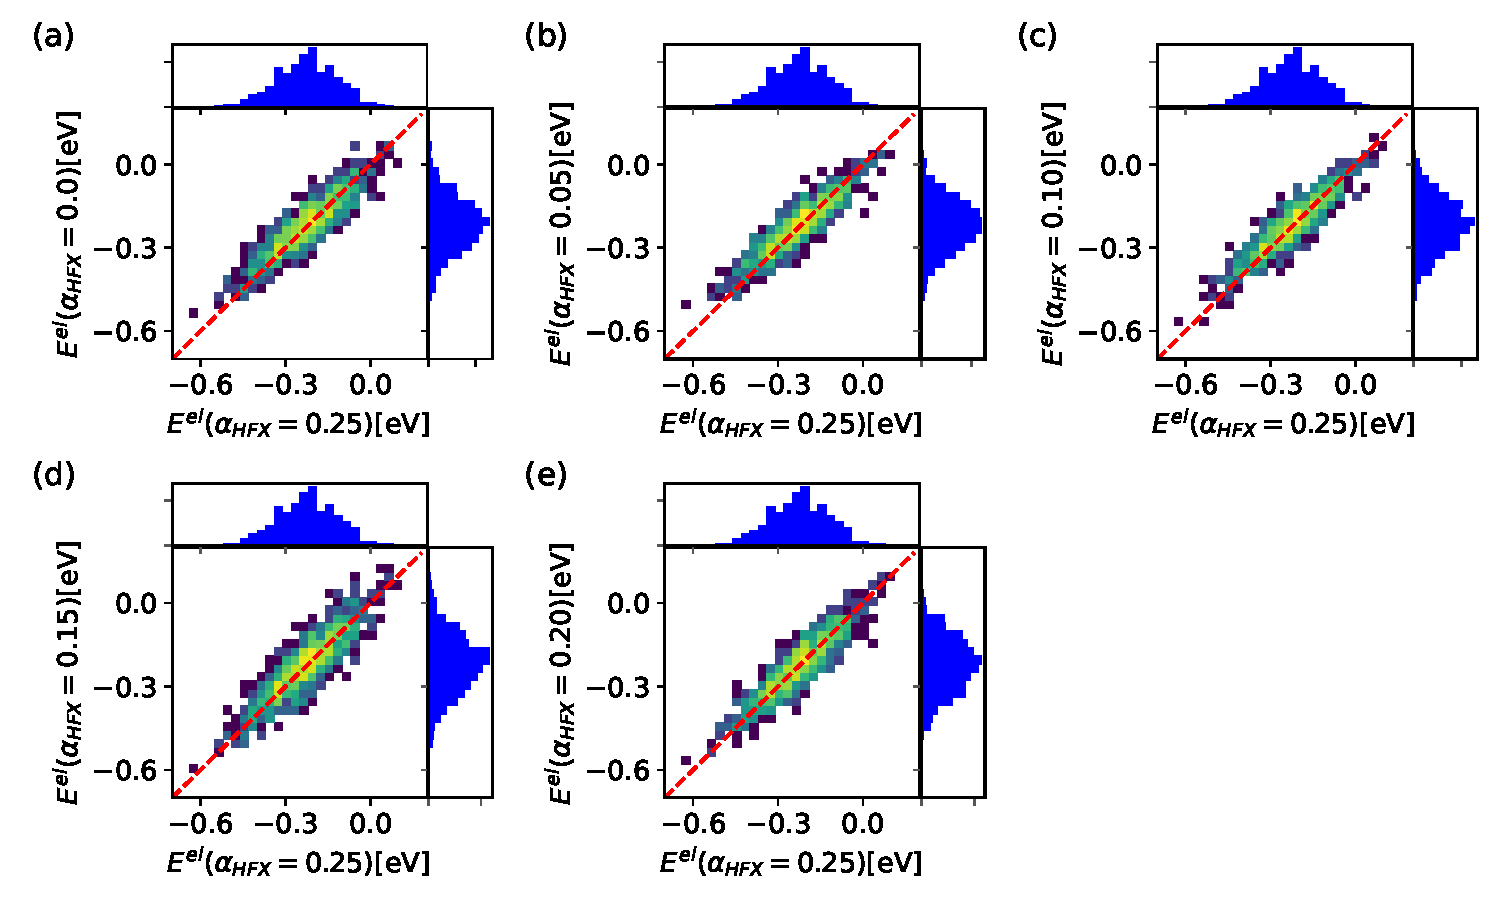
\includegraphics[width=0.80\textwidth]{figs/scatterEstat_qmmm.pdf}
  \caption{\bjoern{TODO Zhong:}{add labels (a)...; replace $\alpha$ with $\alpha_\text{HF}$.}Scatter plot of MADN electrostatic energy calculated from different HFX, compared to the electrostatic energy calculated from HFX=0.25 (The PBE0 functional). The brighter color near the diagonal lines indicates denser population of the molecules.  The top and right histogram show the energy distributions.}
  \label{fig:Estat_qmmm_MADN}
\end{figure*}

\begin{figure*}
  \centering
  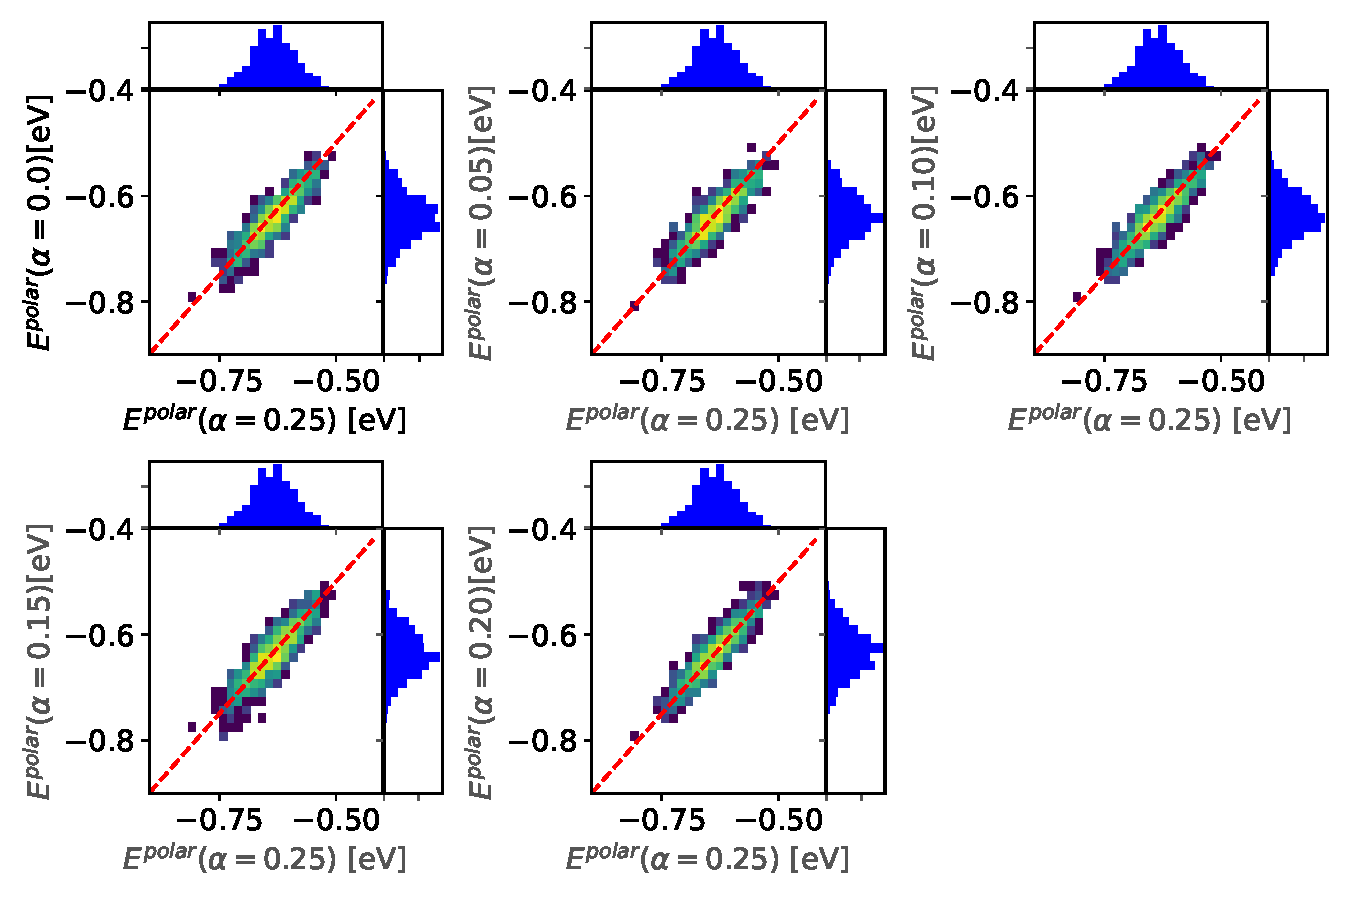
\includegraphics[width=0.80\textwidth]{figs/scatterEdip_qmmm.pdf}
  \caption{\bjoern{TODO Zhong:}{add labels (a)...; replace $\alpha$ with $\alpha_\text{HF}$.}Scatter plot of MADN polarization energy calculated from different HFX, compared to the polarization energy calculated from HFX=0.25 (The PBE0 functional). The brighter color near the diagonal lines indicates denser population of the molecules.  The top and right histogram show the energy distributions.}
  \label{fig:Edip_qmmm_MADN}
\end{figure*}


\end{document}
